\documentclass[aoas,preprint]{imsart}

\RequirePackage[OT1]{fontenc}
\RequirePackage{amsthm,amsmath}
\RequirePackage[numbers]{natbib}
\RequirePackage[colorlinks,citecolor=blue,urlcolor=blue]{hyperref}

\usepackage{graphicx}
\usepackage{algorithm}
\usepackage{algpseudocode}

\usepackage{amssymb,amsmath,amsthm,amsfonts}
\usepackage{mathrsfs}
\usepackage{dsfont}
\usepackage{enumerate}

%\newtheorem{mdef}{Definition}
%\newtheorem{theorem}{Theorem}
\newcommand{\eqsplit}[2]{
  \begin{equation}\label{#2}
    \begin{split}
      #1
    \end{split}
  \end{equation}}
\newcommand{\eqnsplit}[1]{
  \begin{eqnarray*}
    #1
  \end{eqnarray*}}
\newcommand{\tran}[1]{
  \tilde{#1}
}
\newcommand{\td}[2]{
  \frac{d #1}{d #2}
}
\newcommand{\pd}[2]{
  \frac{\partial #1}{\partial #2}
}
\newcommand{\ppd}[2]{
  \frac{\partial^2 #1}{\partial #2^2}
}
\newcommand{\pdd}[3]{
  \frac{\partial^2 #1}{\partial #2 \partial #3}
}
\newcommand{\otd}[1]{
  \frac{d}{d #1}
}
\newcommand{\opd}[1]{
  \frac{\partial}{\partial #1}
}
\newcommand{\oppd}[1]{
  \frac{\partial^2}{\partial #1^2}
}
\newcommand{\opdd}[2]{
  \frac{\partial^2}{\partial #1 \partial #2}
}
\newcommand{\ket}[1]{
  |#1\rangle
}
\newcommand{\bra}[1]{
  \langle#1|
}
\newcommand{\inn}[1]{
  \langle#1\rangle
}
\newcommand{\mean}[1]{
  \langle#1\rangle
}
\newcommand{\tr}{
  \text{tr}\,
}
\newcommand{\re}{
  \text{Re}\,
}
\newcommand\im{
  \text{Im}\,
}
\newcommand{\var}{
  \text{var}
}
\newcommand{\arcsinh}{
  \sinh^{-1}
}
\newcommand{\arccosh}{
  \cosh^{-1}
}
\newcommand{\erfc}{
  \text{erfc}
}
\newcommand{\E}{
  \mathbb{E}
}
\renewcommand{\P}{
  \mathbb{P}
}
\newcommand{\I}[1]{
  \mathbf{1}_{\{#1\}}
}
\newcommand{\1}[1]{
  \mathds{1}_{\{#1\}}
}
\newcommand{\diag}{
  \text{diag\,}
}
\newcommand{\M}{
  {\text{max}}
}
\newcommand{\m}{
  {\text{min}}
}
\newcommand{\ph}{
  {\text{arg}\,}
}
\newcommand\erf{
  \text{erf}
}
\renewcommand\vec[1]{
  \mathbf{#1}
}
\newcommand\mtx[1]{
  \mathbf{#1}
}
\newcommand\ed{
  \,{\buildrel d \over =}\,
}




% settings
%\pubyear{2005}
%\volume{0}
%\issue{0}
%\firstpage{1}
%\lastpage{8}
\arxiv{arXiv:0000.0000}

\startlocaldefs
\numberwithin{equation}{section}
\theoremstyle{plain}
\newtheorem{thm}{Theorem}[section]
\endlocaldefs

\begin{document}

\begin{frontmatter}
\title{Rare event simulation for GARCH(p,q) processes\thanksref{T1}}
\runtitle{Rare event simulation for GARCH(p,q) processes}
\thankstext{T1}{Footnote to the title with the ``thankstext'' command.}

\begin{aug}
\author{\fnms{First} \snm{Author}\thanksref{t1,t2,m1}\ead[label=e1]{first@somewhere.com}},
\author{\fnms{Second} \snm{Author}\thanksref{t3,m1,m2}\ead[label=e2]{second@somewhere.com}}
\and
\author{\fnms{Third} \snm{Author}\thanksref{t1,m2}
\ead[label=e3]{third@somewhere.com}
\ead[label=u1,url]{http://www.foo.com}}

\thankstext{t1}{Some comment}
\thankstext{t2}{First supporter of the project}
\thankstext{t3}{Second supporter of the project}
\runauthor{F. Author et al.}

\affiliation{Copenhagen University\thanksmark{m1} and Another University\thanksmark{m2}}

\address{Address of the First and Second authors\\
Usually a few lines long\\
\printead{e1}\\
\phantom{E-mail:\ }\printead*{e2}}

\address{Address of the Third author\\
Usually a few lines long\\
Usually a few lines long\\
\printead{e3}\\
\printead{u1}}
\end{aug}

\begin{abstract}
The abstract should summarize the contents of the paper.
It should be clear, descriptive, self-explanatory and not longer
than 200 words. It should also be suitable for publication in
abstracting services. Please avoid using math formulas as much as possible.

This is a sample input file.  Comparing it with the output it
generates can show you how to produce a simple document of
your own.
\end{abstract}

\begin{keyword}[class=MSC]
\kwd[Primary ]{60K35}
\kwd{60K35}
\kwd[; secondary ]{60K35}
\end{keyword}

\begin{keyword}
\kwd{sample}
\kwd{\LaTeXe}
\end{keyword}

\end{frontmatter}

\section{Introduction}
Ever since its proposition by Bollerslev~\cite{bollerslev:1986} and
Taylor~\cite{taylor:2008} (cf. also Andersen et al
\cite{andersen:davis:kreiss:mikosch:2009}), the GARCH 
({\em Generalized Autoregressive Conditional Heteroscedasticity}) model
has seen wide-spread application in finance and economics, and has
inspired numerous variants such as GJR-GARCH of Glosten et
al~\cite{glosten:1993}, {\em Asymmetric} GARCH of Engle and
Ng~\cite{engle:Ng:1993} and the {\em Quadratic} GARCH of
Sentana~\cite{sentana:1995}, among others. The basic GARCH model of
Bollerslev~\cite{bollerslev:1986} and Taylor~\cite{taylor:2008}
defines the conditional variance via the stochastic recurrence
equation
\begin{eqnarray}
  R_t &=& \sigma_t Z_t \nonumber \\
  \sigma_{t}^2 &=& \omega + \sum_{i=1}^p \alpha_i R_{t-i}^2 + \sum_{j=1}^q
  \beta_j \sigma_{t-j}^2   \label{eq:garchpq}
\end{eqnarray}
where $\{R_t\}_{t \in \mathbb Z}$ is the return series in question;
$\{Z_t\}_{t \in \mathbb Z}$ is an iid sequence of random variables
with zero mean and unit variance; the distribution function of $Z_t$
is assumed to have a density.
$\omega, \alpha_i, i \in \{1,\dots,p\}$ and
$\beta_j, j \in \{1,\dots,q\}$ are constant parameters. A process
defined by \eqref{eq:garchpq} is called a GARCH($p,q$) process.
When $p = q = 1$,
\[
\sigma_t^2 = \omega + (\alpha_1 Z_{t-1}^2 + \beta_1) \sigma_{t-1}^2
\]
When $p > 1$ or $q > 1$, a matrix recurrence equation arises
(cf. Davis and Mikosch~\cite{davis:mikosch:2001})
\begin{small}
  \begin{equation*}
    \underbrace{
      \begin{pmatrix}
        \sigma_{t}^2 \\
        \sigma_{t-1}^2 \\
        \vdots \\
        \sigma_{t-q+2}^2 \\
        \sigma_{t-q+1}^2 \\
        R_{t-1}^2 \\
        R_{t-2}^2 \\
        \vdots \\
        R_{t-p+2}^2 \\
        R_{t-p+1}^2
      \end{pmatrix}}_{V_t} =
    \underbrace{
      \begin{pmatrix}
        \alpha_1 Z_{t-1}^2 + \beta_1 & \beta_2 & \cdots &
        \beta_{q-1} & \beta_q & \alpha_2 & \alpha_3 & \cdots & \alpha_p & 0 \\
        1 & 0 & \cdots & 
        0 & 0 & 0 & 0 & \cdots & 0 & 0 \\
        \vdots & \vdots & \ddots & 
        \vdots & \vdots & \vdots & \vdots & \ddots & \vdots & \vdots \\
        0 & 0 & \cdots &
        0 & 0 & 0 & 0 & \cdots & 0 & 0 \\
        0 & 0 & \cdots &
        1 & 0 & 0 & 0 & \cdots & 0 & 0 \\
        Z_{t-1}^2 & 0 & \cdots &
        0 & 0 & 0 & 0 & \cdots & 0 & 0 \\
        0 & 0 & \cdots &
        0 & 0 & 1 & 0 & \cdots & 0 & 0 \\
        \vdots & \vdots & \ddots &
        \vdots & \vdots & \vdots & \vdots & \ddots & \vdots & \vdots \\
        0 & 0 & \cdots &
        0 & 0 & 0 & 0 & \cdots & 0 & 0 \\    
        0 & 0 & \cdots &
        0 & 0 & 0 & 0 & \cdots & 1 & 0 \\    
      \end{pmatrix}
    }_{A_t}
    \underbrace{
      \begin{pmatrix}
        \sigma_{t-1}^2 \\
        \sigma_{t-2}^2 \\
        \vdots \\
        \sigma_{t-q+1}^2 \\
        \sigma_{t-q}^2 \\
        R_{t-2}^2 \\
        R_{t-3}^2 \\
        \vdots \\
        R_{t-p+1}^2 \\
        R_{t-p}^2
      \end{pmatrix}
    }_{V_{t-1}} +
    \underbrace{
      \begin{pmatrix}
        \omega \\
        0 \\
        \vdots \\
        0 \\
        0 \\
        0 \\
        0 \\
        \vdots \\
        0 \\
        0 \\
      \end{pmatrix}
    }_{B}
  \end{equation*}
\end{small}
For convenience, define $d = p + q - 1$ and we shall write the above
recurrence equation as
\begin{equation}
  \label{eq:garchpq_sre}
  V_t = A_t V_{t-1} + B
\end{equation}
where $V_t$ and $B$ are $d$-dimensional vectors, $A_t$ are
$d \times d$ matrices. Their definitions are obvious from the above
equation. Notice that for all $t$, $\vec 0 \neq V_t$. Let
$\underline V = \inf_{t \geq 0} |V_t|$. Then $\underline V > 0$.

It is also useful to note that, if given $V_t$ and $V_{t-1}$,
$Z_{t-1}^2$ can be easily found:
\[
z_{t-1}^2 = {
  \inn{\vec e_{q+1}, V_{t}}
  \over
  \inn{\vec e_1, V_{t-1}}
}
\]
where $\inn{\cdot, \cdot}$ denotes the inner product of two vectors.
Since $Z_1, Z_2, \dots$ are iid, so are $A_1, A_2, \dots$.
Let $Z \overset{d}{=} Z_1$ and $A \overset{d}{=} A_1$.
Bollerslev \cite{bollerslev:1986} showed that the fixed-point
stochastic equation $X \overset{d}{=} A X + B$ has a unique, strictly
stationary solution with finite variance if and only if
\begin{equation}
  \sum_{i=1}^p \alpha_i + \sum_{j=1}^q \beta_j < 1
  \label{eq:bollerslev}
\end{equation}
In the rest of this paper, we always assume condition
\eqref{eq:bollerslev} is satisfied. For convenience of narration, let
$\pi$ denote this unique stationary probability measure and let
$V \sim \pi$, $Z \sim \mu_Z$. More generally we write $\mu_U$ for the
probability measure of $U$, no matter what type of object $U$ may be.

According to Buraczewski et al 
\cite{buraczewski:damek:mikosch:2016}, proposition 4.3.1, the support
of $\pi$ is
\[
\chi = \overline{
  \left\{
  (I_{p+q-1} - a)^{-1} b:
  \exists n \geq 1,
  a = \prod_{i=1}^n A_i,
  \|a\| < 1,
  b = \left(\sum_{i=0}^{n-1} \prod_{j=1}^i A_{j}\right) B,
  \right\}
}
\]
where $\overline S$ denotes the closure of set $S$.
In addition to \eqref{eq:bollerslev}, we assume the following about
the recurrence equation \eqref{eq:garchpq_sre}:
\begin{enumerate}[(I)]
\item $\exists s > 0$ such that
  $1 < \E (\alpha_1 Z^2 + \beta_1)^s < \infty$
\item If $p, q \geq 2$, there exists an non-empty open set
  $S \subset \supp \mu_Z$.
\end{enumerate}
Clearly, these conditions are satisfied when $Z$ has normal or $t$
distributions.
Before proceeding any further, it is worthwhile to point out a few
implications of the above assumptions:
\begin{enumerate}[(i)]
\item \eqref{eq:garchpq} immediately implies
  \[
  \sigma_t^2 \geq \omega \left(
    1 - \sum_{j=1}^q \beta_j
  \right)^{-1} = \sigma_{\m}^2
  \]
  Then it follows
  $\chi \subseteq [\sigma_{\m}^2, \infty)^q \times [0, \infty)^{p-1}$, so
  $V_n \in \chi$ for all $n \geq 0$. Since the random variable
  $Z_{n-1}^2$ is assumed to have a continuously differentiable
  distribution function,
  $\P(Z_{n-1}^2 = x) = 0$ for all $x \in \text{supp } \mu_{Z^2}$.
  Furthermore, $Z_{n-1}^2$ uniquely determines the matrix $A_n$,
  so it follows $\P(A v + B = v) = 0$ for all $v \in \chi$.

\item \eqref{eq:bollerslev} implies the top Lyapunov exponent of $A_n$
  \[
  \gamma = \inf_{n \geq 1} {1 \over n} \E \left(\log \| A_n \cdots A_1 \| \right)
  \]
  is negative. Cf. Buraczewski et al
  \cite{buraczewski:damek:mikosch:2016}, prop. 4.1.12.

\item That $\vec 0 \notin \chi$ and $A_n$ has a Lebesgue density implies
  the stationary distribution $\pi$ is absolutely continuous with
  respect to Lebesgue measure. This immediately follows from lemma
  4.2.2 of Buraczewski et al \cite{buraczewski:damek:mikosch:2016}.
\end{enumerate}
The implications (i), (ii), (iii) are in fact the conditions of
proposition 4.2.1 of Buraczewski et al
\cite{buraczewski:damek:mikosch:2016}, from which we conclude $V_n$ is
an aperiodic, positive Harris chain that is in addition
$\pi$-irreducible on $\chi$.
Moreover, from (I) it follows $0 < \exists \xi < s$ such that
\begin{equation}
  \label{eq:hyt}
  \lambda(\xi) = \lim_{n \to \infty} (\E \|A_n \cdots A_1\|^\xi)^{1/n} = 1
\end{equation}
and
\begin{equation}
  \label{eq:jui}
  \E \|A\|^\xi < \infty
\end{equation}
The existence of $\xi$ together with Conditions (ii) and (II)
allow the application of Kesten-Goldie theorem (cf. Buraczewski et al
\cite{buraczewski:damek:mikosch:2016}, example 4.4.13). Here and in
the rest of this paper, we use $\tilde V$ to denote $V/|V|$, $V'$ to
denote the transpose of $V$ for a vector $V$,
and $\tilde S$ to denote $\{\tilde v: v \in S\}$ for a set $S$.

The Kesten-Goldie theorem gives
\begin{equation}
  \label{eq:kesten}
  \lim_{x \to \infty} x^{\xi} \P(\tilde y' V > u) = e_\xi(\tilde y)  
\end{equation}
for some function $e_\xi: \tilde \chi \to \reals_+$ and
all $\tilde y \in \tilde \chi$. Here $d = p + q - 1$ and $\tilde y'$
is the transpose of $\tilde y$. Cf. Kesten \cite{kesten:1973} and
Buraczewski et al \cite{buraczewski:damek:mikosch:2016},
section 4.4.4.

Although the probability $\P(\tilde y' V > u)$ has been given
asymptotically by the Kesten-Goldie theorem, one often wishes to know
this probability more precisely, due to the importance of risk
management. Now that more detailed analytic description of the
probability is unknown, one has to resort to numerical methods. But
the occurrence of $\tilde y' V > u$ for a large $x$ is a rare event; a
naive Monte-Carlo approach will be very inefficient. Cf. Asmussen and
Glynn \cite{opac-b1123521}.
One way to increase the efficiency of Monte-Carlo methods is
importance sampling. To our best knowledge, no importance sampling
estimator has been proposed in the literature for the computation of
$\P(\tilde y' V > u)$ or for the more general problem when the
defining recurrence equation of $V_n$ i.e. \eqref{eq:garchpq_sre} is 
more general than that of GARCH($p, q$). We present a solution in this
paper.

When $p = q = 1$, $V_n$ reduces to a scalar. An importance sampling
estimator was proposed and shown to be efficient in the sense of
bounded relative error by Collamore et al \cite{collamore2014}. We
consider our work as a multivariate extension to theirs.

% \section{Statement of the Problem}
% We intend to find an estimator of bounded relative error for the
% probability $\P(\tilde y' V > u)$. But before we introduce the
% estimator we would like to point out a few properties of the
% GARCH($p,q$) process which will be essential for the estimator.
% For convenience of description, let $\chi$ denote the state space of
% the Markov chain $V_n$.

% For this purpose, we use a
% result of Collamore and Mentemeier \cite{collamore:mentemeier:2016},
% who showed that, under the following conditions, the chain $V_n = A_n
% V_{n-1} + B_n$, not necessarily a GARCH($p, q$) process, is an
% aperiodic positive Harris chain on $\reals_+^d = \{x \in \mathbb
% R^d: \forall i  = 1,\dots, d,\; \inn{e_i, x} \geq 0\}$. Here
% $\{e_1, \dots, e_d\}$ denote a orthonormal basis of $\reals^d$ and
% $\inn{\cdot, \cdot}$ denotes inner product (cf. lemma 3.4 of
% \cite{collamore:mentemeier:2016})
% \begin{enumerate}[(i)]
% \item For each and every $n \geq 1$ and for all
%   $1 \leq i \leq j \leq d$, $(A_n)_{i,j} \geq 0$.
% \item With probability 1, the matrices $A_n$ have no all-zero rows or
%   columns, i.e.
%   \[
%   \P \left\{
%   \text{$\exists 1 \leq i \leq n$ such that
%     $\forall 1 \leq j \leq n$, $(A_n)_{i,j} = 0$ or $(A_n)_{j,i} = 0$
%   }
%   \right\} = 0
%   \]
% \item The additive subgroup of $\reals$ generated by
%   \[
%   \{\log \rho(\Pi): \Pi = \prod_{i=1}^n A_i \quad \text{for some n
%     and iid. } A_i\}.
%   \]
%   is dense in $\reals$. Here $\rho(\Pi)$ denotes the largest
%   singular value of $\Pi$.
% \item $\exists \xi > 0$ such that $\lambda(\xi) = 1$, where
%   \[
%   \lambda(\xi) := \inf_{n \geq 1} (\E \|A_n \cdots A_1\|^\xi)^{1/n}
%    \]
%   \end{eqnarray*}
% \item Let $\pi$ denote the stationary distribution of $V_n$ and $P$
%   denote the transition kernel of $V_n$. Assume that
%   there exists a set $\mathcal C$ with $\pi(\mathcal C) > 0$
%   such that $\forall x \in \mathcal C$, $P(x, \cdot)$ has an
%   absolutely continuous component with respect to some $\sigma$-finite
%   non-null measure $\phi$.
% \end{enumerate}

% It is straightforward to verify these conditions for a GARCH($p, q$)
% process. Conditions (i) and (ii) are obvious.

% Moreover, it follows from condition (v)
% \[
% P(x, A) \geq \I_{\mathcal C}(x) \phi(A) \inf_{y \in A} f(y)
% \]
% where $f(\cdot)$ is the Radon-Nikodym derivative of $P(x, \cdot)$ with
% respect to $\phi$. This minorization condition gives rise to a
% regenerative structure of the path of $V_n$. Cf. Ney and Nummelin
% \cite{ney:nummelin:1987}, lemma 3.1. Let $\tau$ has the distribution of
% the length of a regeneration cycle in this structure.
Now we introduce a {\em Markov Additive} process $(X_n, S_n)$
associated with the Markov chain $V_n$:
\begin{eqnarray*}
X_n &=& {
        A_n A_{n-1} \cdots A_1 \tilde V_0
        \over
        |A_n A_{n-1} \cdots A_1 \tilde V_0|
      }, \quad X_0 = \tilde V_0\\
S_n &=& \log |A_n \cdots A_1 \tilde V_0| \\
\l_n &=& S_n - S_{n-1} = \log |A_n X_{n-1}|
\end{eqnarray*}
Define mapping
\[
g: (x, y, l) \in \sphere^{d-1} \times \sphere^{d-1} \times \reals
\to
\reals_+ \ni {
  \inn{\vec e_{q+1}, e^l y}
  \over
  \inn{\vec e_{1}, x}
}
\]
Then $Z_{n-1}^2 = g(X_{n-1}, X_n, l_n)$. Let
\[
\mathscr F_n = \mathcal B(X_0, X_1, \dots, X_n, l_1, l_2, \dots, l_n)
\]
where $\mathcal B(\cdot)$ denotes the $\sigma$-field generated by
$\cdot$. It is clear $\mathcal B(V_n) \subseteq \mathscr F_n$.
Let $P$ denote the transition kernel of $(X_n, S_n)$. We have
\[
  P(x, dy \times dl) = \P(X_n \in dy, l_n \in dl | X_{n-1} = x)
  = \P(Z_{n-1}^2 \in g(x, dy, dl))
  \]
Note $g(\sphere^{d-1}, \sphere^{d-1}, \reals) = \img Z^2$,
where $\img Z^2$ denotes the image of $Z^2$.
Choose a set $\mathcal S \subset \sphere^{d-1}$ such that
\[
\inf_{w \in g(\mathcal S, \sphere^{d-1}, \reals)} f_{Z^2}(w) > 0
\]
We have
\begin{eqnarray*}
  P(x, dy \times dl) \geq
  \I_{\mathcal S}(x) \inf_{w \in g(\mathcal S, dy, dl)} f_{Z^2}(w)
  | g(\mathcal S, dy, dl)| 
\end{eqnarray*}
where $f_{Z^2}(\cdot)$ is the density function of $Z^2$ with respect to the
Lebesgue meausure and $|\cdot|$ denotes the Lebesgue measure. It is
easy to see
\[
\int_{\sphere^{d-1} \times \reals} \inf_{w \in g(\mathcal S, dy, dl)} f_{Z^2}(w)
| g(\mathcal S, dy, dl)| < \infty
\]
Clearly
\begin{eqnarray*}
  &&
  \int_{\sphere^{d-1} \times \reals} \inf_{w \in g(\mathcal S, dy, dl)} f_{Z^2}(w)
  | g(\mathcal S, dy, dl)| \\
  &\leq&
  \int_{\sphere^{d-1} \times \reals}
  \int_{g(\mathcal S, dy, dl)} f_{Z^2}(w) dw \\
  &=&
  \int_{g(\mathcal S, \sphere^{d-1}, \reals)} f_{Z^2}(w) dw \\
  &<&
  \int_{\img Z^2} f_{Z^2}(w) dw = 1
\end{eqnarray*}
Let
\[
\delta = \int_{\sphere^{d-1} \times \reals}
\inf_{w \in g(\mathcal S, dy, dl)} f_{Z^2}(w)
| g(\mathcal S, dy, dl)| < 1
\]
and
\[
\nu(dy \times dl) = {1 \over \delta}
\inf_{w \in g(\mathcal S, dy, dl)} f_{Z^2}(w)
| g(\mathcal S, dy, dl)|
\]
Now that $\nu(\sphere^{d-1} \times \reals) = 1$, $\nu(\cdot)$ is a
probability measure. We have the minorization condition
\begin{equation}
  \label{eq:minorization}
  P(x, dy \times dl) \geq \delta \I_{\mathcal S}(x) \nu(dy \times dl)
\end{equation}
By Ney and Nummelin \cite{ney:nummelin:1987}, lemma 3.1,
\eqref{eq:minorization} implies the MA-process $(X_n, S_n)$ has a
regenerative structure:
\begin{enumerate}[(1)]
\item There exist random variables $0 < \tau_0 < \tau_1 < \dots$,
  $i = 0, 1, 2, \dots$ such that $\tau_{i+1} - \tau_i$,  are iid.
\item The blocks
  \[
  (X_{\tau_i}, X_{\tau_i + 1}, \dots, X_{\tau_{i+1} - 1}, l_{\tau_i},
  l_{\tau_i + 1}, \dots, l_{\tau_{i+1} - 1}) \quad
  i = 0, 1, 2, \dots
  \]
  are independent of each other.
\item
  \[
  \P[(X_{\tau_i}, l_{\tau_i}) \in S \times \Gamma | \mathscr F_{\tau_i - 1}]
  = \nu(S \times \Gamma)
  \]
\end{enumerate}
Furthermore, \eqref{eq:minorization} means
$P(x, dy \times dl)$ can be decomposed as
\[
P(x, dy \times dl) = P'(dx, dy \times dl)
+
\delta \I_{\mathcal S}(x) \nu(dy \times dl)
\]
Thus the MA-process regenerates only when it is in $\mathcal S$ and in
this case it regenerates with probability $\delta$. That is
\[
\P[(X_n, S_n) \text{ regenerates } | X_{n-1} = x] = \delta \I_{\mathcal S}(x)
\]
There is yet another useful property of the iid matrices $A_n$. Define
mapping
\[
A \cdotp x: (A, x) \in \img(A) \times \sphere^{d-1} \to
\sphere^{d-1} \ni {
  A x \over |A x|
}
\]
and operator $\mathscr P_\theta$ for $\theta \in \reals$,
$f: \sphere^{d-1} \to \reals_+$:
\[
\mathscr P_\theta f(x) =
\E \left[
  |A x|^\theta f(A \cdotp x)
\right]
\]
By Lemma 2.2 of Collamore and Mentemeier
\cite{collamore:mentemeier:2016}, \eqref{eq:jui} means
$\lambda(\xi) = 1$ is the spectral radius of $\mathscr P_\xi$ and
there is a unique, strictly positive eigen function $r_\xi(\cdot)$
associated with $\lambda(\xi)$ i.e.
$\mathscr P_\xi r_\xi(x) = \lambda(\xi) r_\xi(x)$.
Moreover, $r_\xi$ is $\max\{\xi, 1\}$-H\"older continuous, implying
$r_\xi$ is bounded from above and below by positive constants. From
now on, we use the notations
\[
\bar r_\xi = \sup_{x \in \sphere^{d-1}} r_\xi(x),\quad
\underline r_\xi = \inf_{x \in \sphere^{d-1}} r_\xi(x)
\]

There is also an eigen measure $\ell_\xi$ on $\mathcal B(\sphere^{d-1})$
associated with the operator
$\mathscr P_\xi$ that corresponds to the eigen value
$\lambda(\xi) = 1$ and eigen function $r_\xi$:
\[
\E \left[ |A x|^\xi \ell(A \cdotp dx) \right]
= \ell_\xi \mathscr P_\xi (dx)
= \lambda(\xi) \ell_\xi(dx)
\]
The eigen function $r_\xi$ and eigen measure $\ell_\xi$ are called
right eigen function and left eigen measure, respectively. They
satisfy the identity
$\ell_\xi r_\xi = \int_{\sphere^{d-1}} r_\xi(x) \ell_\xi(dx) = 1$.
Cf. Collamore and Mentemeier \cite{collamore:mentemeier:2016},
Lemma 2.2.

When $\E \|A\|^\theta < \infty$, we define a shifted probability
measure $\mu_A^\theta$ on $\mathcal B(\text{dom}(A))$:
\[
\mu_A^\theta(S) = {
  \E [ \| A \|^\theta \I_S(A)]
  \over
  \E \|A\|^\theta
}
\]
Accordingly, we denote the expectation taken with respect to
$\mu_A^\theta$ as $\E_\theta$, in which we omit the marking of $A$
whose involvment should be obvious from the context.
Now we extend the definition of the operator $\mathscr P$ by replacing
the expectation taken with respect to the original measure with the
expectation taken with respect to the shifted measure, i.e. we
define
\[
\mathscr P_{\varphi, \theta} f(x)
= \E_\varphi \left[
  |A x|^\theta f(A \cdotp x)
\right], \quad
\eta \mathscr P_{\varphi, \theta}(dx)
=
\E_\varphi \left[ |A x|^\theta \eta(A \cdotp dx) \right]
\]
where $f$ is a function $f: \sphere^{d-1} \to \reals$ and
$\eta$ is a probability measure on $\mathcal B(\sphere^{d-1})$.
By Lemma 2.2 of Collamore and Mentemeier
\cite{collamore:mentemeier:2016}, when
$\E_\varphi \| A \|^\theta < \infty$, the spectral radius of
$\mathscr P_{\varphi, \theta}$ is
\[
\lambda_\varphi(\theta) = \lim_{n \to \infty}
\left(\E_\varphi \|A_n \cdots A_1 \|^\theta\right)^{1/n}
\]
and a unique pair of eigen function and eigen measure exists
for $\mathscr P_{\varphi, \theta}$ corresponding to
$\lambda_\varphi(\theta)$. Call them
$r_{\varphi, \theta}(\cdot)$ and $\ell_{\varphi, \theta}(\cdot)$,
respectively.

Naively one would estimate $\P(|V| > u)$ as
$n^{-1} \sum_{i=1}^n \1{|V_i| > u}$, applying the law of large
numbers. The difficulty with this naive method is that, when $u$ is
large, $|V_i| > u$ happens very rarely, resulting in a large variance
of the estimator. To tackle this problem, we use importance sampling
and exponentially shift the transition kernel of the MA process
$(X_i, S_i)$, i.e. the conditional probability $P(x, dy \times dl)$,
until $|V_t| > u$. Let
\[
P_\theta(x, dy \times dl)
=
{e^{\theta l} \over \lambda(\theta)}
{r_\theta(y) \over r_\theta(x)}
P(x, dy \times dl)
\]
Since the matrix $A_t$ depends only on $Z_{t-1}^2$, shifting the
transition kernel of $(X_t, S_t)$ is equivalent to shifting the
conditional distribution of $Z_{t-1}^2$. It follows from the above
equation
\[
{
  \P_\theta(Z_{t-1}^2 \in dw | X_{t-1} = x)
  \over
  \P(Z_{t-1}^2 \in dw | X_{t-1} = x)
} = {|A(w) x|^\theta \over \lambda(\theta)}
{
  r_\theta (A(w) \cdotp x)
  \over
  r_\theta(x)
}
\]
where $\P_\theta(\cdot | \cdot)$ denotes the shifted conditional
probability measure.

% Once the threshold $u$ has been exceeded by $|V_t|$, we change the
% the distribution of $Z^2$ and hence the transition kernel of the
% MA-process back to their original, since the process is recurrent
% under the original kernel.
Now we are ready to introduce our importance sampling estimator.
We start the process from within
$\mathcal C = \{v \in \chi: |v| \leq M\}$ i.e.
$V_0 \in \mathcal C$
and let $V_0 \sim \gamma$, where the probability
measure $\gamma$ is defined as
\[
\gamma(S) = \pi(S) / \pi(\mathcal C)
\quad \forall S \in \mathcal B(\mathcal C)
\]
Let $K_0 = 0$,
$K_1 = \inf\{n > 0: |V_n| \leq M\}$ and
$K_i = \inf\{n > K_{i-1}: |V_n| \leq M\}$.
These are the times of the $V_n$ chain returning to the set
$\mathcal C$. Define
\begin{eqnarray*}
  R_n &:=& \sup\{i \geq 0: K_i \leq n\} \\
%%  K &\overset{d}{=}& K_{i+1} - K_i\quad i = 0, 1, 2, \dots \\
  T_u &=& \inf\{n \geq 1: |V_n| > u\} \\
  N_u &:=& \sum_{i=0}^{K_1 - 1} \1{V_i > u} \\
  \mathcal E_u &=& \pi(\mathcal C)
  N_u \1{T_u < K_1} e^{-\xi S_{T_u}}
  {r_\xi(X_0) \over r_\xi(X_{T_u})}
\end{eqnarray*}
$\mathcal E_u$ is our estimator. We have
\begin{equation}
  \label{eq:fbf}
  \P(|V| > u) = \E_{\mathcal D} \mathcal E_u
\end{equation}
where the subscript $\mathcal D$, short for ``dual'', is to remind us
that the expectation is taken with respect to the shifted kernel
$P_\xi$ before the threshold is exceeded, and with respect to the
original kernel $P$ thereafter.
%% The following notations are used:
%% \begin{eqnarray*}
%%   %% R_n &:=& \sup\{i \geq 0: K_i \leq n\} \\
%%    &\overset{d}{=}& K_{i+1} - K_i\quad i = 0, 1, 2, \dots \\
%%   T_u &=& \inf\{n \geq 1: |V_n| > u\} \\
%%   N_u &:=& \sum_{i=1}^\tau \1{V_i > u}
%% \end{eqnarray*}
In \S\ref{sec:drift} we show that, with certain shifted kernels, the
MA-process drifts towards a set of bounded $|V_t|$. This is a crutial
fact for the consistency and efficiency of $\mathcal E_u$.
Then in \S\ref{sec:consistency} we prove the relation \eqref{eq:fbf} and in
\S\ref{sec:efficiency} we prove that the estimator $\mathcal E_u$ is
efficient i.e. its relative error is bounded.

\section[The Chain Drifts towards a Small Set]{$V_n$ Drifts towards a Small Set}\label{sec:drift}
\begin{lemma}
  Let $\varphi \in \reals$ satisfy
  \begin{equation}
    \label{eq:drift_cond}
    \E \|A\|^\varphi < \infty,\quad\text{ and }
    \inf_{\theta > 0} {\E \|A\|^{\theta + \varphi}
      \over 
      \E \|A\|^{\varphi}
    } < 1
  \end{equation}
  then there exist $\theta > 0$ such that
  $\E_\varphi \|A\|^\theta < 1$ 
  and $0 < b < 1, M > 0$ such that
  \begin{equation}
    \label{eq:drift}
    \E_\varphi \left[\left.
      |V_n|^\theta r_{\varphi, \theta}(\tilde V_n)
      \1{|V_{n-1}| > M} \right|
      \mathscr F_{n-1} \right]
    \leq
    b |V_{n-1}|^\theta
    r_{\varphi, \theta}(\tilde V_{n-1})
  \end{equation}
  where the expectation $E_\varphi$ is taken with respect to
  $\mu_A^\varphi$.
\end{lemma}

\begin{proof}
  By condition \eqref{eq:drift_cond}, there is a $\theta > 0$ such
  that $\E_\varphi \|A\|^\theta < 1$, because
  \[
  \E_\varphi \|A\|^\theta
  =
  \int \|\mtx a\|^\theta {
    \|\mtx a \|^\varphi \mu_A (d\mtx a)
    \over
    \E \|A\|^{\varphi}
  }
  = {
    \E \|A\|^{\varphi + \theta}
    \over
    \E \|A\|^{\varphi}    
  }
  \]
  Then, by lemma 2.2 of Collamore and Mentemeier
  \cite{collamore:mentemeier:2016}, a unique eigen
  function $r_{\varphi, \theta}(\cdot)$ and a unique eigen measure
  $ \ell_{\varphi, \theta}(\cdot)$ exist for $\mathscr P_{\varphi,
    \theta}$.
  Thus, with the operator $\mathscr P^*_{\varphi, \theta}$ adjoint to
  $\mathscr P_{\varphi, \theta}$ defined analogously as in Collamore
  and Mentemeier, the right eigen function $r_{\varphi, \theta}(x)$
  can be represented as
  \[
  r_{\varphi, \theta}(x) = c \int_{\sphere^{d-1}} \inn{x, y}^\theta
  d\ell^*_{\varphi, \theta}(y)
  \]
  We have
  \begin{eqnarray}
    && \E_\varphi \left[ |V_n|^\theta r_{\varphi, \theta}(\tilde V_n)
      \1{|V_{n-1}| > M} | \mathscr F_{n-1} \right]
    \nonumber \\
    &=&
    \1{|V_{n-1}| > M}
    \E_\varphi\left[\int_{\sphere^{d-1}} \inn{V_n, y}^\theta d\ell^*_{\varphi,\theta}(y)|
      \mathscr F_{n-1} \right]
    \nonumber \\
    &=&
    \1{|V_{n-1}| > M}
    \E_\varphi\left[\int_{\sphere^{d-1}} (\inn{A_n V_{n-1}, y} + \inn{B,
        y})^\theta d\ell^*_{\varphi,\theta}(y) | \mathscr F_{n-1} \right]
    \label{eq:drift_proof_1}
  \end{eqnarray}
  \begin{enumerate}
  \item if $\theta \leq 1$, by subadditivity we have
    \begin{eqnarray*}
      &&\E_\varphi\left[\int_{\sphere^{d-1}} (\inn{A_n V_{n-1}, y} + \inn{B,
          y})^\theta d\ell^*_{\varphi,\theta}(y) | \mathscr F_{n-1} \right]\\
      &\leq& \E_\varphi\left[\int_{\sphere^{d-1}} \inn{A_n V_{n-1}, y}^\theta
        d\ell^*_{\varphi,\theta}(y) | \mathscr F_{n-1} \right]
      + \E_\varphi\left[\int_{\sphere^{d-1}} \inn{B, y}^\theta d\ell^*_{\varphi,\theta}(y) |
        \mathscr F_{n-1} \right] \\
      &=& \E_\varphi\left[|V_{n-1}|^\theta |A_n \tilde V_{n-1}|^\theta\int_{\sphere^{d-1}}
        \inn{ A_n \cdotp \tilde V_{n-1}, y}^\theta
        d\ell^*_{\varphi,\theta}(y) | \mathscr F_{n-1} \right]  + |B|^\theta r_{\varphi,\theta}(\tilde B)\\
      &=& |V_{n-1}|^\theta  \int |\mathbf a \tilde V_{n-1}|^\theta
      r_{\varphi, \theta}(\mathbf a \cdotp \tilde V_{n-1})
      d\mu_A^\varphi (\mathbf a) + |B|^\theta r_{\varphi,\theta}(\tilde B) \\
      &=&
      |V_{n-1}|^\theta (
      \mathscr P_{\varphi, \theta}
      r_{\varphi, \theta})(\tilde V_{n-1}) + |B|^\theta r_{\varphi,\theta}(\tilde B) \\
      &=& |V_{n-1}|^\theta r_{\varphi, \theta}(\tilde V_{n-1}) \lambda_\varphi(\theta)
      \left\{
        1 + 
        {|B|^\theta r_{\varphi, \theta}(\tilde B)
          \over
          |V_{n-1}|^\theta \lambda_\varphi(\theta) r_{\varphi,
            \theta}(\tilde V_{n-1})
        }
        \right\} \\
    \end{eqnarray*}
    By lemma 2.2 of Collamore and Mentemeier
    \cite{collamore:mentemeier:2016}, $r_{\varphi, \theta}$ is bounded
    from above and below. Therefore the last equation gives
    \begin{eqnarray*}
      && \E_\varphi \left[ \left.
        |V_n|^\theta r_{\varphi, \theta}(\tilde V_n) \1{|V_{n-1}| > M}
        \right| \mathscr F_{n-1}
        \right] \\
      &<&
      |V_{n-1}|^\theta r_{\varphi, \theta}(\tilde V_{n-1})
      \underbrace{
        \lambda_\varphi(\theta)
        \left[
          1 + 
          {
            |B|^\theta r_{\varphi,\theta}(\tilde B)
            \over
            M^\theta \lambda_\varphi(\theta)
            \underline r_{\varphi, \theta}
          }
          \right]
      }_{b}
      \1{|V_{n-1}| > M} \\
      &\leq&
      |V_{n-1}|^\theta r_{\varphi, \theta}(\tilde V_{n-1}) b
    \end{eqnarray*}
    Note
    \[
    \lambda_\varphi(\theta)
    =
    \left(
    \E_\varphi \| A_n \cdots A_1 \|^\theta
    \right)^{1/n}
    \leq
    \left(
    \E_\varphi (\| A_1 \|^\theta)^n
    \right)^{1/n}
    =
    \E_\varphi \| A_1 \|^\theta  <  1
    \]
    If $M$ satisfies
    \[
    M >
    \left\{
     |B|^\theta r_{\varphi, \theta}(\tilde B)
    \over
    [1 - \lambda_\varphi(\theta)] \underline r_{\varphi, \theta}
    \right\}^{1/\theta}
    \]
    we have $b < 1$ and \eqref{eq:drift} holds.

  \item If $\theta > 1$, applying Minkowski's inequality to the RHS
      of \eqref{eq:drift_proof_1} and using similar arguments as in
      the previous case gives
      \begin{eqnarray*}
        && \E_\varphi \left[ \left.
          |V_n|^\theta r_{\varphi, \theta}(\tilde V_{n})
          \1{|V_{n-1}| > M}
          \right| \mathscr F_{n-1}
        \right] \\
        &\leq&
        |V_{n-1}|^\theta r_{\varphi, \theta}(\tilde V_{n-1})
        \underbrace{
        \lambda_\varphi(\theta) \left\{
          1 + \left[
            {
              |B|^\theta r_{\varphi,\theta}(\tilde B)
              \over
              M^\theta
              \underline r_{\varphi, \theta}
              \lambda_\varphi(\theta)
            }
          \right]^{1/\theta}
          \right\}^\theta
          }_{b}
          \1{|V_{n-1}| > M}
      \end{eqnarray*}
      and correspondingly, $M$ needs to satisfy
      \begin{equation*}
        M > \left[
          {
            r_{\varphi,\theta}(\tilde B) |B|^\theta
            \over
            \underline r_{\varphi, \theta}
          }
        \right]^{1/\theta} {
          1 \over
          1 - \lambda_\varphi(\theta)^{1/\theta}
        }
      \end{equation*}
      so that $b < 1$. This proves \eqref{eq:drift}.
  \end{enumerate}    
\end{proof}

\begin{remark}
  \label{remark:1}
  Iterating \eqref{eq:drift} yields, for $j \geq 0, n > 1$
  \[
  \E_\varphi \left[
    \left.
    |V_{K_j + n}|^\theta r_{\varphi, \theta}(\tilde V_{K_j + n})
    \prod_{i=1}^{n-1}\1{|V_{K_j + i}| > M}
    \right| \mathscr F_{K_j + 1}
    \right]
  \leq b^{n-1} |V_{K_j + 1}|^\theta r_{\varphi, \theta}(\tilde V_{K_j+1})
  \]
  Because
  $\{K_{j+1} - K_j > n - 1\} \subseteq \bigcap_{i=K_j + 1}^{K_j + n-1}\{|V_i| > M\}$,
  \begin{eqnarray*}
  \E_\varphi \left[\left.
    |V_{K_j + n}|^\theta \underline r_{\varphi, \theta}
    \1{K_{j+1} - K_j > n - 1}
    \right| \mathscr F_{K_j + 1}
    \right]
  &\leq&
  b^{n-1} |V_{K_j + 1}|^\theta \bar r_{\varphi, \theta} \\
  \E_\varphi \left[
    |V_{K_j + n}|^\theta \underline r_{\varphi, \theta}
    \1{K_{j+1} - K_j > n - 1}
    \right]
  &\leq&
  b^{n-1} \E_\varphi |V_{K_j + 1}|^\theta \bar r_{\varphi, \theta}
  \end{eqnarray*}
  Moreover,
  \[
  \E_\varphi |V_{K_j + 1}|^\theta
  \leq
  \E_\varphi \|A_{K_j + 1}\|^\theta |V_{K_j}|^\theta + |B|^\theta
  \leq
  M^\theta + |B|^\theta
  \]
  So we have
  \[
  \P_\varphi(K_{j + 1} - K_j > n-1)
  \leq
  b^{n-1} \rho(\varphi, \theta)
  \]
  for a constant
  \[
  \rho(\varphi, \theta) = {
    \bar r_{\varphi,\theta}
    \over
    \underline r_{\varphi,\theta}
  } {
    M^\theta + |B|^\theta
    \over
    \underline V^\theta
  }
  \]
  Since for each $\varphi$ the inequality holds for all
  $\theta$ satisfying
  $\E \|A\|^{\varphi + \theta} < \E \|A\|^\varphi$,
  we have for $n \geq 1$,
  \[
  \P_\varphi (K_{j+1} - K_j> n)
  \leq
  \left( \sup_{\theta \in \Theta(\varphi)} b(\varphi, \theta) \right)^n
  \sup_{\theta \in \Theta(\varphi), b(\varphi, \theta) < 1}
  \rho(\varphi, \theta)
  = b_\varphi^n \rho_\varphi
  \]
  where
  $\Theta(\varphi) = \{\theta: \E \|A\|^{\varphi + \theta} < \E \|A\|^\varphi\}$,
  and $b_\varphi < 1$.
\end{remark}

\section{The Estimator is Unbiased}\label{sec:consistency}
\begin{theorem}
  The estimator $\mathcal E_u$ is unbiased, i.e. equation
  \eqref{eq:fbf} holds.
\end{theorem}
\begin{proof}
  By the {\em strong law of large numbers} for Markov chains,
  \begin{eqnarray*}
    {1 \over n} \sum_{i=0}^n \1{|V_i| > u} \overset{a.s.}{\to} \P(|V| > u)
  \end{eqnarray*}
  Define $R_n =\sup\{i \geq 0: K_i \leq n\}$. Then one can write
  \begin{eqnarray}
    {1 \over n} \sum_{i=1}^n \1{|V_i| > u}
    &=& 
    {1 \over n} \left[
      \sum_{i=0}^{K_{R_n}-1} \1{|V_i| > u} + \sum_{i=K_{R_n}}^n \1{|V_i| > u}
    \right]
    \label{eq:kioj}
  \end{eqnarray}
  For the 2nd term on the right side, we show in the following
  \begin{equation}
    \label{eq:frf}
    {1 \over n}\sum_{i=K_{R_n}}^n \1{|V_i| > u} \overset{a.s.}{\to} 0
  \end{equation}
  This is, by definition, for all $\epsilon > 0$
  \begin{eqnarray*}
    \P \left[
      \bigcup_{N=1}^\infty \bigcap_{n=N}^\infty
      \left\{
        {1 \over n} \sum_{i=K_{R_n}}^{n} \1{|V_i| > u} \leq \epsilon
      \right\}
    \right] &=& 1 \\
    \P \left[
      \bigcap_{N=1}^\infty \bigcup_{n=N}^\infty
      \left\{
        {1 \over n} \sum_{i=K_{R_n}}^{n} \1{|V_i| > u} > \epsilon
      \right\}
    \right] &=& 0 \\
  \end{eqnarray*}
  By Borel-Cantelli lemma, it suffices to show
  \[
  \sum_{n=1}^\infty \P\left[
    {1 \over n} \sum_{i=K_{R_n}}^{n} \1{|V_i| > u} > \epsilon
  \right] < \infty
  \]
  Clearly
  \begin{eqnarray*}
    && \sum_{n=1}^\infty \P\left[
      {1 \over n} \sum_{i=K_{R_n}}^{n} \1{|V_i| > u} > \epsilon
    \right] \\
    &\leq&
    \sum_{n=1}^\infty \P\left[
      {1 \over n} \sum_{i=K_{R_n}}^{K_{R_n + 1} - 1} \1{|V_i| > u} > \epsilon
    \right] \\
    &\leq&
    \sum_{n=1}^\infty \P\left(
      {K_{R_n + 1} - K_{R_n}} > \floor{\epsilon n}
    \right)
  \end{eqnarray*}
  It suffices to show
  \[
  \sum_{n=\ceil{1/\epsilon}}^\infty \P\left(
    {K_{R_n + 1} - K_{R_n}} > \floor{\epsilon n}
  \right) < \infty
  \]
  By Remark \ref{remark:1} with $\varphi = 0$,
  $\P(K_{j + 1} - K_j > k) < b_0^n \rho_0$ for $k \geq 1$.
  Thus
  \[
    \sum_{n=\ceil{1/\epsilon}}^\infty \P\left(
    {K_{R_n + 1} - K_{R_n}} > \floor{\epsilon n}
  \right)
  <
  \sum_{n=\ceil{1/\epsilon}}^\infty b_0^{\floor{\epsilon n}} \rho_0 < \infty
  \]
  This shows \eqref{eq:frf} holds.
  For the 1st term on the right side of \eqref{eq:kioj}, we have
  \[
  {1 \over n} \sum_{i=0}^{K_{R_n}-1} \1{|V_i| > u}
    =
    {R_n \over n} {1 \over R_n} \sum_{i=1}^{R_n}
    \sum_{j=K_{i-1}}^{K_i-1}\1{|V_i| > u}
  \]
  It can be shown $(V_{K_i}, \sum_{j=K_{i-1}}^{K_i-1}\1{|V_i| > u})$
  is a positive Harris chain. Moreover
  \[
  \E \left(
    \sum_{j=K_{i-1}}^{K_i-1}\1{|V_i| > u}
  \right)
  \leq
  \E (K_i - K_{i-1}) < \sum_{n=1}^\infty n b_0^n \rho_0 < \infty
  \]
  Therefore, by the law of large numbers for Markov chains,
  \begin{eqnarray*}
    {R_n \over n} {1 \over R_n} \sum_{i=1}^{R_n}
    \sum_{j=K_{i-1}}^{K_i-1}\1{|V_i| > u}
    &\overset{a.s.}{\to}& \pi(\mathcal C) \E_\gamma N_u
  \end{eqnarray*}
  On the other hand, by the very definition of $N_u$,
  $\E_\gamma N_u = \E_\gamma \left( N_u \1{T_u < K_1}\right)$. We have
  \begin{small}
    \begin{eqnarray*}
      && \E_\gamma \left( N_u \1{T_u < K_1}\right) \\
      &=&
      \underbrace{
        \int_{\sphere^{d-1}} \int_{\reals}
        \cdots
        \int_{\sphere^{d-1}} \int_{\reals}
      }_{K_1 - 1\text{ folds}}
      N_u \1{T_u < \tau}
      \prod_{i=1}^{T_u} e^{-\xi l_i}
      {r_\xi(x_{i-1}) \over r_\xi(x_{i})}P_\xi(x_{i-1}, dx_i \times dl_i)
      \prod_{i=T_u+1}^{K_1 - 1} P(x_{i-1}, dx_i \times d l_i) \\
      &=&
      \E_{\mathcal D}
      \left[
        N_u \1{T_u < K_1} e^{-\xi S_{T_u}}
        {r_\xi(X_0)
          \over
          r_\xi(X_{T_u})
        }
      \right]
    \end{eqnarray*}
  \end{small}
  Thus we have proved the theorem.
\end{proof}

\section{The Estimator Has Bounded Relative Error}\label{sec:efficiency}

\begin{theorem}
  The estimator $\mathcal E_u$ has bounded relative error, i.e.
  \begin{equation*}
    \limsup_{u \to \infty} {\var(\mathcal E_u) \over [\P(|V| > u)]^2} < \infty
  \end{equation*}
\end{theorem}
\begin{proof}
  The assertion is equivalent to
  \[
  \limsup_{u \to \infty} {\E_{\mathcal D} \mathcal E_u^2 \over [\P(|V|
    > u)]^2} < \infty
  \]
  By Kesten's theorem \cite{kesten:1973}, $\P(|V| > u) \sim C
  u^{-\xi}$. Hence, to prove the assertion, one needs to check
  $\limsup_{u \to \infty} u^{2\xi}\E_{\mathcal D} \mathcal E_u^2 <
  \infty$, i.e.
  \[
  \limsup_{u \to \infty} \E_{\mathcal D}
  \left[
    u^{2\xi}
    N_u^2 \1{T_u < K_1} e^{-2\xi S_{T_u}} {r_\xi^2(X_0)
      \over r_\xi^2(X_{T_u})}
  \right] < \infty
 \]
 We note $V_t = \sum_{n=0}^t A_{t} \cdots A_{n+1} B$ and
 $|V_{T_u}| > u$. Moreover $r_\xi$ is bounded
 from above and below by positive constants. So it suffices to show
 \begin{eqnarray}
   f(\xi) &=& \limsup_{u \to \infty} \E_{\mathcal D} \left[
     \left|
       \sum_{n=0}^{T_u}
       \frac{
         N_u^{1/\xi} A_{T_u} \cdots A_{n+1} B 
       }{
         |A_{T_u} \cdots A_1 X_0|
       }
       \1{T_u < K_1}
     \right|^{2 \xi}
   \right] < \infty \label{eq:efficiency_target}
 \end{eqnarray}
  In the rest of the proof, we write $c, c_1, c_2, \dots$ for
  constants whose values have no importance and depend on the
  context. If $\xi > 1$, Minkowski's inequality gives
    \begin{eqnarray*}
      f(\xi) &\leq& \limsup_{u \to \infty}
      \left\{
        \sum_{n=0}^{\infty}
        \left[
          \E_{\mathcal D} \left|
            N_u^{1/\xi}
            \frac{
              A_{T_u} \cdots A_{n+1} B 
            }{
              |A_{T_u} \cdots A_1 X_0|
            }
            \1{n \leq T_u < K_1}
          \right|^{2 \xi}
        \right]^{1/2\xi}
      \right\}^{2\xi} \nonumber \\
      f(\xi)
      &\leq&
      c \limsup_{u \to \infty}
      \left\{
      \sum_{n=0}^\infty
      \left(
        \E_D {
          \|A_{T_u} \cdots A_{n+1}\|^{2\xi}
          \1{n \leq T_u < K_1}
          N_u^2
          \over
          |A_{T_u} \cdots A_{n+1} X_n|^{2\xi}
          |A_n \cdots A_1 X_0|^{2\xi}
        }
        \right)^{1/2\xi}
        \right\}^{2\xi}\\
      &\leq&
      c \limsup_{u \to \infty}
      \sum_{n=0}^\infty
      \left(
        \E_D |A_n \cdots A_1 X_0|^{-2\xi}
        N_u^2
        \1{n \leq T_u < K_1}        
      \right)^{1/2\xi} \\
      &\leq&
      c \limsup_{u \to \infty}
      \sum_{n=0}^\infty
      \E \left(
        |A_n \cdots A_1 X_0|^{-\xi}
        N_u^2
        \1{n \leq T_u < K_1}        
      \right)^{1/2\xi} \label{eq:split_point}
    \end{eqnarray*}
    
  \begin{enumerate}
  \item If $\lambda(-\xi) < \infty$, we assume
    \begin{equation}
      \label{eq:cond1}
      \lambda(-\xi)
      \inf_{\alpha \in \reals} \lambda_{-\xi}(\alpha) < 1
    \end{equation}
    Changing to the $-\xi$-shifted measure, we obtain
    \begin{eqnarray*}
      &&
      c \sum_{n=0}^\infty
      \E \left(
        |A_n \cdots A_1 X_0|^{-\xi}
        N_u^2
        \1{n \leq T_u < K_1}        
      \right)^{1/2\xi} \\
      &\leq&
      c \sum_{n=0}^\infty
      \E_{-\xi} (N_u^2 \1{n \leq T_u < K_1})
      \lambda(-\xi)^n \\
      &\leq&
      c \sum_{n=0}^\infty
      \E_{-\xi} (K_1^2 \1{n < K_1})
      \lambda(-\xi)^n \\
      &\leq&
      c \sum_{n=0}^\infty
      \sum_{l=n+1}^\infty
      l^2 \P_{-\xi}(K_1 > l-1)
      \lambda(-\xi)^n
    \end{eqnarray*}
    Applying Remark \ref{remark:1} with $\varphi = -\xi$ gives, for some
    $a > 0$, $\P_{-\xi}(K_1 > l-1) \leq a [\delta \lambda_{-\xi}(\alpha)]^{l-2}$
    for all $\delta > 1$ and $\delta \lambda_{-\xi}(\alpha) < 1$
    provided that $M$ is chosen sufficiently large. Thus the RHS of the
    above inequality is bounded by
    \begin{eqnarray*}
      c \sum_{n=0}^\infty
      \lambda(-\xi)^n
      \sum_{l=n+1}^\infty
      l^2 [\delta \lambda_{-\xi}(\alpha)]^{l-2}
    \end{eqnarray*}
    The second sum in the above evaluates to a finite sum of terms
    each having the form $c n^k [\delta
    \lambda_{-\xi}(\alpha)]^n$. Hence to show $f(\xi) < \infty$, it
    suffices to show
    \begin{equation*}
      \sum_{n=0}^\infty
      n^k [\delta \lambda(-\xi) \lambda_{-\xi}(\alpha)]^n < \infty
    \end{equation*}
    Under assumption \eqref{eq:cond1} the above inequality is
    obviously true.
  \item If $\lambda(-\xi) = \infty$, we assume $\lambda(h\xi) <
    \infty$ and $\E(|B|/\|A\|)^{h\xi} <  \infty$. Since
    \[
    V_n = \sum_{i=0}^n A_n \cdots A_{i+1} B
    \]
    it follows
    \begin{eqnarray*}
      |V_n|\1{K_1 > n} &\leq&
      \sum_{i=0}^{n} \|A_n \cdots A_{i+1}\| |B| \\
      \|A_n \cdots A_1\|^{-1} \1{K_1 > n}
      &\leq& |V_n|^{-1} \1{K_1 > n}
      \left[
        |B_0| + \sum_{i=1}^n {
          \|A_n \cdots A_{i+1}\|
          \over
          \|A_n \cdots A_{1}\|
        } |B|
      \right] \\
      &\leq& {1 \over M}
      \left[
        |B_0| + \sum_{i=1}^n {
          \|A_n \cdots A_{i+1}\|
          \over
          \|A_n \cdots A_{1}\|
        } |B| \1{K_1 > n}
      \right]
    \end{eqnarray*}
    Note
    \[
    \|A_n \dots A_{i+1} A_i \cdots A_1\| \geq
    C^{-1} \|A_n \cdots A_{i+1}\|
    \|A_i \cdots A_{1}\|
    \]
    for some $C > 1$. We have
    \begin{equation}
      \label{eq:lower_bound}
      \|A_n \cdots A_1\|^{-1} \1{K_1 > n}
      \leq
      {1 \over M} \left[
        |B_0| + \sum_{i=1}^n {
          C |B|
          \over
          \|A_i \cdots A_1\|
        }  \1{K_1 > n}
      \right]
    \end{equation}
    Let
    \[
    J_k = \|A_k \cdots A_1\|^{-1} \1{K_1 > n}
    \]
    We obtain
    \begin{eqnarray*}
      \left(
        \E J_n^\zeta
      \right)^{1/\zeta} &\leq& \left[
        \E \left(
          {|B_0| \over M}
          + {C \over M} \sum_{i=1}^n |B| J_i
        \right)^\zeta
        \right]^{1/\zeta}
    \end{eqnarray*}
    Using Minkowski's inequality and the independence of $B$ and
    $A_i, \dots, A_1$ the above yields
    \begin{eqnarray}
      (\E J_n^\zeta)^{1/\zeta} &\leq&
      {|B_0| \over M} + {C \over M}
      \sum_{i=1}^n
      (\E |B|^\zeta)^{1/\zeta}
      (\E J_i^\zeta)^{1/\zeta}
      \label{eq:neg_pow_ub} \\
      &=& h_1 + h_2 \sum_{i=1}^{n-1} (\E J_i^\zeta)^{1/\zeta}
      \nonumber
    \end{eqnarray}
    where
    \begin{eqnarray*}
      h_1 &=& {|B_0| \over M} \\
      h_2 &=& {C \over M} (\E |B_1|^\zeta)^{1/\zeta}
    \end{eqnarray*}
    Since
    \begin{eqnarray*}
      V_1 &=& A_1 V_0 + B_1 \\
      |V_1| &\leq& \|A_1\| |V_0| + |B_1| \\
      \end{eqnarray*}
      and by assumption $\E (|B|/\|A\|)^\zeta < \infty$, we have
      \begin{eqnarray}
        (\E J_1^\zeta)^{1/\zeta} &=&
        \left[
        \E (\|A_1\|^{-\zeta}\1{K_1 > n})
      \right]^{1/\zeta} \nonumber \\
      &\leq&
      {|V_0|\over M} \E \left[\left(
        1 + {|B_1| \over |V_0| \|A_1\|}
      \right)^\zeta
      \1{K_1 > n}\right]^{1/\zeta}< \infty
    \label{eq:J_1}
    \end{eqnarray}
    Let
    \[
    y_1(\zeta) = 
    {|V_0|\over M} \E \left[\left(
        1 + {|B_1| \over |V_0| \|A_1\|}
      \right)^\zeta \1{K_1 > n}\right]^{1/\zeta}
    \]
    and
    \begin{equation}
      \label{eq:y_n}
      y_n(\zeta) = h_1 + h_2 \sum_{i=1}^{n-1} y_i(\zeta)
    \end{equation}
    Then \eqref{eq:neg_pow_ub}, \eqref{eq:y_n} and \eqref{eq:J_1}
    yield
    \begin{equation}
      \label{eq:J_n_2}
      (\E J_n^\zeta)^{1/\zeta} \leq y_n(\zeta)
    \end{equation}
    Meanwhile \eqref{eq:y_n} gives, $\forall n \geq 1$,
    \begin{equation}
      \label{eq:y_n_2}
      y_n(\zeta) = {y_1(\zeta) \over (1 - h_2)^{n-1}}
    \end{equation}

    Now from \eqref{eq:split_point} it follows by H\"older's inequality
    \begin{eqnarray*}
      f(\xi)^{1/2\xi}
      &\leq&
      c \sum_{n=0}^\infty
      (\E N_u^{2r})^{1/r}
      (\E |A_n \cdots A_1 X_0|^{-s\xi}\1{n \leq T_u < K_1})^{1/s} \\
      &\leq&
      c \sum_{n=0}^\infty
      (\E K_1^{2r})^{1/r}
      (\E |A_n \cdots A_1 X_0|^{-s\xi}\1{n \leq T_u < K_1})^{1/s}
    \end{eqnarray*}
    where $1/r + 1/s = 1$. Obviously
    \begin{eqnarray*}
      \E K_1^{2r}
      &\leq&
      \sum_{l=2}^\infty l^{2r} \P(K_1 > l-1)
    \end{eqnarray*}
    Applying Remark \ref{remark:1} with $\beta = 0$ gives $\P(K_1 >
    l-1) \leq a [\delta \lambda(\alpha)]^{l-2}$ for some $a > 0$ and
    all $\delta > 1$ such that $\delta \lambda(\alpha) < 1$. So we
    have
    \begin{eqnarray*}
      \sum_{l=2}^\infty l^{2r} \P(K_1 > l-1) < \infty
    \end{eqnarray*}
    for any finite $r$. Thus it remains to show
    \begin{equation}
      \label{eq:sum_neg_pow}
      \sum_{n=0}^\infty
      (\E |A_n \cdots A_1 X_0|^{-s\xi}\1{n \leq T_u < K_1})^{1/s}
      < \infty
    \end{equation}
    Since for each $n$, it has been shown
    \begin{equation*}
      \E (\|A_n \cdots A_1\|^{-s\xi}\1{n \leq T_u < K_1})
      < y_n(s\xi)^{s\xi} < \infty
    \end{equation*}
    We may choose $L_n > 0$ and $L_n \downarrow 0$ sufficiently fast that
    \begin{equation*}
      \E (
      \|A_n \cdots A_1\|^{-s\xi}
      \I_{F_n^\complement}
      \1{K_1 > n} 
      ) < {1 / n^{s+\epsilon}}
    \end{equation*}
    where $\epsilon > 0$ and
    \begin{equation*}
      F_n = \bigcap_{i=1}^n \{\|A_i\| \geq L_n\}
    \end{equation*}
    Thus
    \begin{equation*}
      \sum_{n=0}^\infty
      (\E |A_n \cdots A_1 X_0|^{-s\xi}\1{n \leq T_u < K_1}
      \I_{F_n^\complement})^{1/s}
      \leq
      1 + 
      \sum_{n=1}^\infty {1 \over n^{(s + \epsilon)/s}} < \infty
    \end{equation*}
    To prove \eqref{eq:sum_neg_pow}, we still have to show
    \begin{equation}
      \label{eq:sum_on_F_n}
      \sum_{n=0}^\infty
      (\E |A_n \cdots A_1 X_0|^{-s\xi}\1{n \leq T_u < K_1}
      \I_{F_n})^{1/s} < \infty
    \end{equation}
    For each matrix $A_n$, construct a matrix $\bar A_{n, k}$, whose
    $(i,j)$-th entry is
    \begin{equation*}
      (\bar A_{n,k})_{i,j} = (A_n)_{i,j}\1{(A_n)_{ij} > L_k} +
      L_n (1 + U_{i,j})\1{(A_n)_{i,j} \leq L_k}
    \end{equation*}
    where $L_k \downarrow 0$ as $k \to \infty$; $U_{i,j}$ are
    iid. and uniformly distributed on $(0,1)$.

    Observe
    \begin{eqnarray*}
      \|\bar A_{n,k}\|
      &=&
      \max_{|x| = 1} |\bar A_{n,k} x| \\
      &\geq&
      \max_{|x| = 1}
      \left|
        \sum_{i=1}^d \left(\sum_{j=1}^d L_k x_j \right)^2
      \right|^{1/2} \\
      &\geq& L_k d^{1/2}
    \end{eqnarray*}
    Hence for any $k < \infty$,
    \begin{eqnarray*}
      {1 \over n}
      \log \E
      \|\bar A_{n,k} \cdots \bar A_{1,k}\|^{-\alpha}
      &\leq&
             {1 \over n} \log \E \left(
             C^{-\alpha(n-1)} \prod_{i=1}^n \|\bar A_{i,k}\|^{-\alpha}
             \right) \\
      &=& {1 \over n} \left[
          -\alpha(n-1) \log C
          + \sum_{i=1}^n \log \E \|\bar A_{i,k}\|^{-\alpha}
          \right] \\
      &\leq&
          -{n - 1 \over n} \alpha \log C
          -\alpha \log (L_k d^{1/2})
    \end{eqnarray*}
    where $C < 1$ is some constant. Cearly the RHS tends to a constant
    as $n \to \infty$. Define
    \begin{equation*}
      \bar \Lambda_{k}(-\alpha) = \sup_{n \geq 1} {1 \over n} \log
      \E\|\bar A_{n,k} \cdots \bar A_{1,k}\|^{-\alpha}
    \end{equation*}
    Since
    \begin{equation*}
      \|\bar A_{n,k} \cdots \bar A_{1,k}\|^{-\alpha}
      \geq
      \|\bar A_{n,k} \cdots \bar A_{i,k}\|^{-\alpha}
      \|\bar A_{n,i-1} \cdots \bar A_{1,k}\|^{-\alpha}
    \end{equation*}
    By Fekete's lemma
    \begin{equation*}
      {1 \over n} \log \E \|\bar A_{n,k} \cdots \bar A_{1,k}\|^{-\alpha}
      \to
      \bar \Lambda_{k}(-\alpha)
    \end{equation*}
    Now consider
    \begin{eqnarray*}
      \bar g_k(\xi) = \sum_{n=0}^\infty
      (\E |\bar A_{n,k} \cdots \bar A_{1,k} X_0|^{-s\xi}
      \1{n \leq \bar T_u < \bar K_1}
      \I_{F_n}
      )^{1/s}
    \end{eqnarray*}
    where $\bar T_u$ and $\bar K_1$ are defined analogously. Changing
    to the $-s\xi$-shifted measure, we obtain
    \begin{eqnarray*}
      \bar g_k(\xi) &=& \sum_{n=0}^\infty \bar \lambda_{k}(-s\xi)^{n/s}
      (\E_{-s\xi} \1{n \leq \bar T_u < \bar K_1} \I_{F_n})^{1/s} \\
      &\leq&
      \sum_{n=0}^\infty \bar \lambda_{k}(-s\xi)^{n/s}
      [\P_{-s\xi}(n \leq \bar T_u < \bar K_1)]^{1/s}
    \end{eqnarray*}
    Applying Remark \ref{remark:1} with $\beta = -s\xi$ gives
    \begin{eqnarray*}
      \P_{-s\xi}(\bar K_1 > n) \leq a [\delta \bar \lambda_{k, -s\xi}(\alpha)]^{n-1}
    \end{eqnarray*}
    for some $a > 0$ and all $\delta > 1$ such that
    $\delta \lambda_k(\alpha - s\xi) < 1$. So we have
    \begin{eqnarray*}
      \bar g_k(\xi) &\leq& 1 + a \bar \lambda_k(-s\xi)\sum_{n=1}^\infty
      [\delta \bar \lambda_{k, -s\xi}(\alpha) \bar \lambda_k(-s\xi)]^{n-1} 
    \end{eqnarray*}
    Note
    \begin{eqnarray*}
      \bar \lambda_{k, -s\xi}(\alpha)
      \leq
      \E_{-s\xi} \bar A_{1,k}^\alpha 
      = {
        \E \bar A_{1,k}^{\alpha - s\xi}
        \over
        \E \bar A_{1,k}^{-s\xi}
      }
      = {
        \bar \lambda_k(\alpha - s\xi)
        \over
        \bar \lambda_k(-s\xi)
      }
    \end{eqnarray*}
    It follows
    \begin{eqnarray*}
      \bar g_k(\xi) &\leq& 1 + \sum_{n=1}^\infty
      [\delta \bar \lambda_k(\alpha - s\xi)]^{(n-1)/s}
      < \infty
    \end{eqnarray*}
    As $k \to \infty$, $\bar g_k(\xi)$ tends to the LHS of
    \eqref{eq:sum_on_F_n} and
    \[
    \delta \bar \lambda_k(\alpha - s\xi) \to \delta \lambda(\alpha - s\xi)
    < 1
    \]
    Thus we conclude \eqref{eq:sum_on_F_n} holds.
    \end{enumerate}
\end{proof}

\section[Estimation of xi]{Estimation of $\xi$}
\subsection{The algorithm}
The idea is to estimate $\Lambda(\alpha)$ according to
\begin{equation}
  \label{eq:Lambda}
  \Lambda(\alpha) = \lim_{n \to \infty}{1 \over n} \log \left(
    \E |A_n \cdots A_1 X_0|^\alpha
  \right)
\end{equation}
and then solve $\Lambda(\xi) = 0$ for $\xi$.
\begin{figure}[htb!]
  \centering
  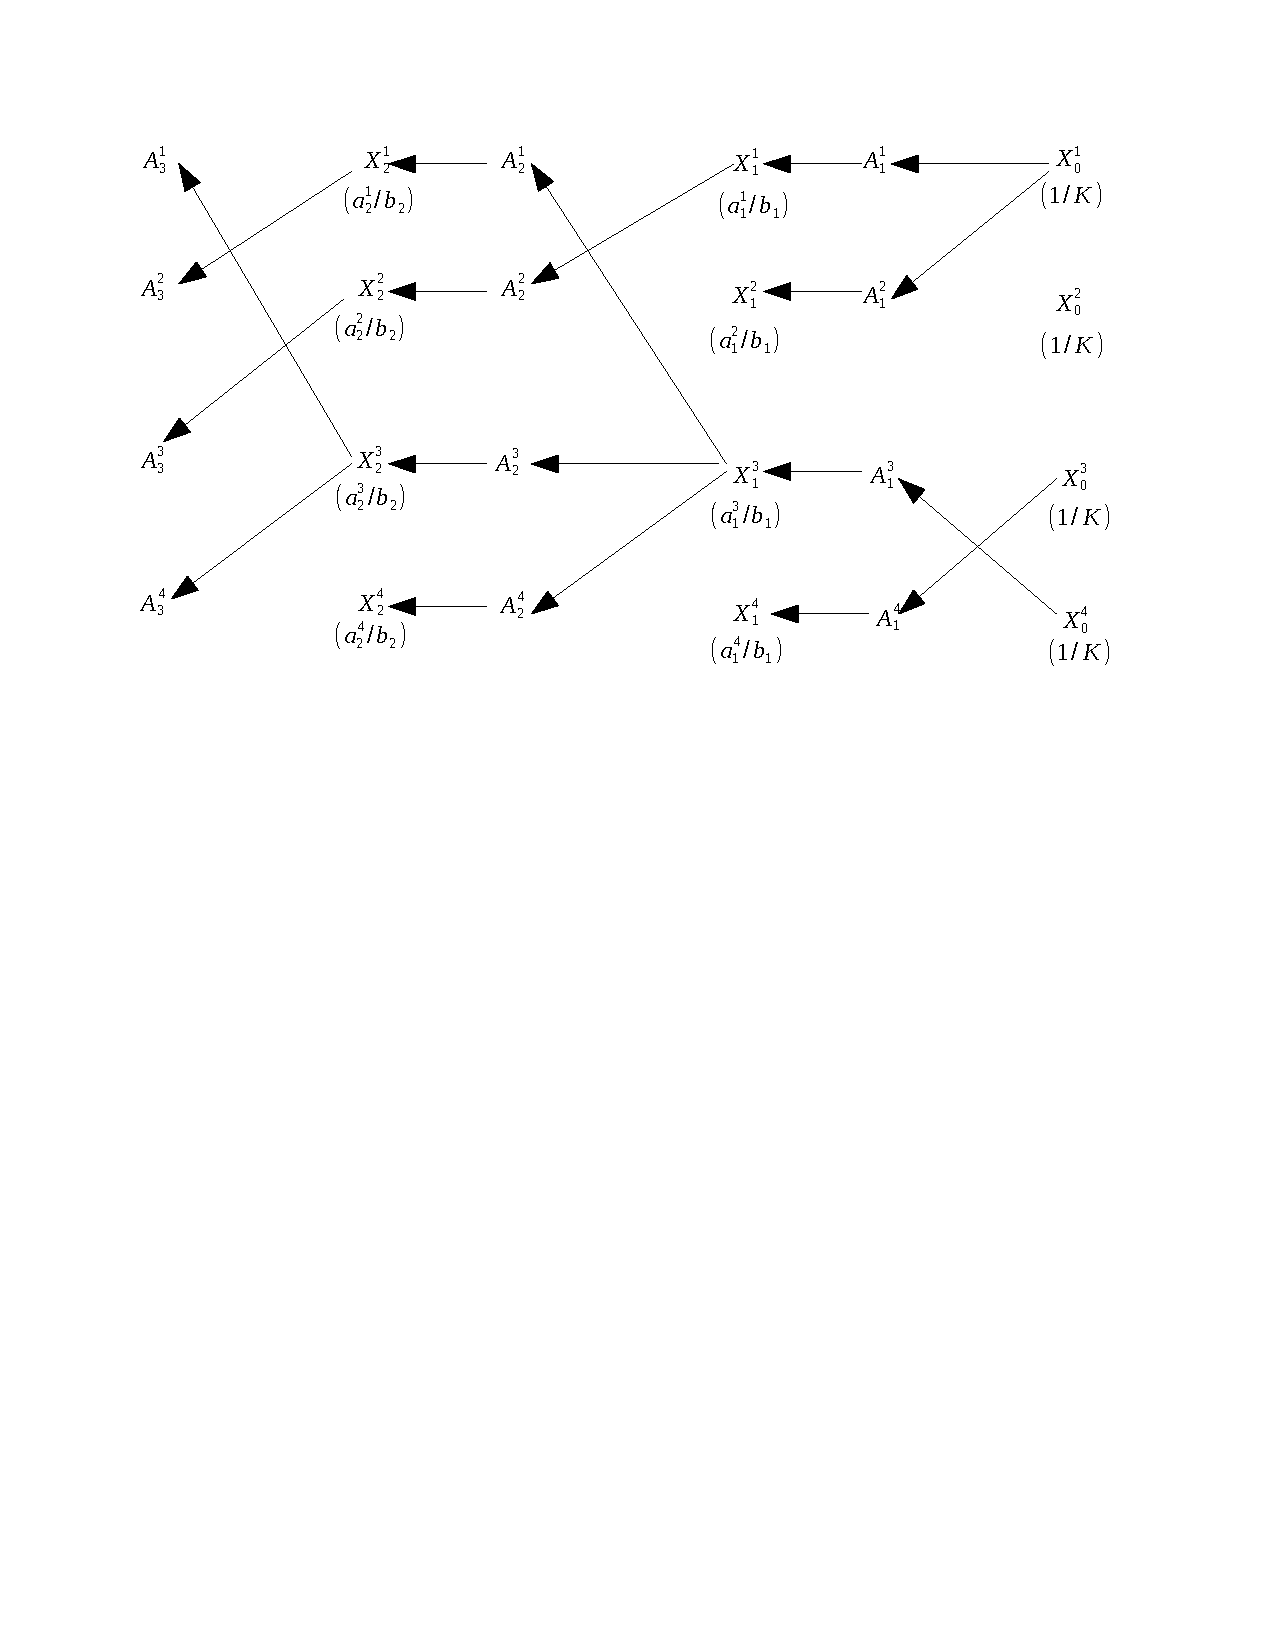
\includegraphics[width=\linewidth, trim=2cm 16cm 2.5cm 2cm, clip]{AnandsEstimator.pdf}
  \caption{A possible realization of the re-sampling procedure. $n =
    3$, $K = 4$. A number in a parenthesis indicates the probability
    of the unit vector above it being chosen to the next step.}
  \label{fig:AnandsEstimator}
\end{figure}
The difficulty with brute-force simulation and estimation is that,
when $n$ is large, the variance of $|A_n \cdots A_1 X_0|^\alpha$
is very large too, resulting in uselessly inaccurate estimations. One
approach of variance reduction is re-sampling. We divide the
estimation of $\Lambda(\alpha)$ into $n$ steps and we are prepared to
simulate $K$ realizations of $A_n, \dots, A_1$ and $X_0$. For
convenience, let
\begin{eqnarray*}
  M_n &=& A_n \cdots A_1 X_0 \\
  X_n &=& {M_n \over |M_n|}
\end{eqnarray*}
We can write
\begin{eqnarray*}
  M_n &=& A_n X_{n - 1} |M_{n - 1}| \\
  &=& A_n X_{n - 1} |A_{n-1} X_{n-2}| \cdot |M_{n-2}| \\
  &=& \cdots \\
  |M_n|^\alpha &=& \prod_{i=1}^n |A_i X_{i-1}|^\alpha
\end{eqnarray*}
With $K$ realizations of $A_n, \dots, A_1$ and $X_0$, a brute-force
estimator of ${1 \over n} \log(\E |M_n|^\alpha)$ can be
\[
{1 \over n} \log \left(
  {1 \over K} \sum_{l=1}^K \prod_{i=1}^n |A_i^l X^l_{i-1}|^\alpha
\right)
\]
where $A_i^l$ denotes the $l$-th realization of $A_i$ and
$X^l_{i-1} = A_{i-1}^l X^l_{i-2}/|A_{i-1}^l X^l_{i-2}|$. To reduce the
variance of the estimator, we introduce a re-sampling procedure:
\begin{equation}
  \label{eq:AnandsEstimator}
  \mathscr E_\alpha =
  {1 \over n}
  \sum_{i=1}^n \log \left(
    {1 \over K}\sum_{l=1}^K |A_i^l X^{w_{l, i-1}}_{i-1}|^\alpha
  \right)
\end{equation}
where the random variable $w_{l, i-1}$ has conditional distribution
\begin{eqnarray*}
  \P(w_{l, i-1} = j | w_{1, i-2}, \dots, w_{K, i-2}) &=& {a^j_{i-1} \over b_{i-1}} \\
  a_{i-1}^j &=& |A_{i-1}^j X_{i-2}^{w_{j, i-2}}|^\alpha \\
  b_{i-1} &=& \sum_{l=1}^K a_{i-1}^l
\end{eqnarray*}
\begin{theorem}
  \[
  \E \left\{
    \sum_{i=1}^n \log \left(
      {1 \over K}\sum_{l=1}^K |A_i^l X^{w_{l, i-1}}_{i-1}|^\alpha
    \right)
  \right\} = \log \left(
    \E |A_n \cdots A_1 X_0|^\alpha
  \right)
  \]
\end{theorem}
Figure \ref{fig:AnandsEstimator} shows a possible realization of the
resampling procedure and algorithm \ref{alg:Lambda_estimation}
outlines an implementation of $\mathscr E_\alpha$. We take
$|\cdot|$ as the max norm.
For an GARCH(p, q) processes, the $A_i$ matrices have dimension
$d \times d$, where $d = p + q - 1$, and the $X_i$ are $d$-dimensional
unit vectors. 
\begin{algorithm}[H]
  \caption{Algorithm for estimating
    $\Lambda(\alpha) = \lim_{n \to \infty} {1 \over n} \log\left(\E |A_n \cdots A_1|^\alpha \right)$}
  \label{alg:Lambda_estimation}
  \begin{algorithmic}
    \Procedure{$\mathscr E_\alpha$}{$n, K$}
    \State Define $K$ $d$-dimensional vectors $X^1, \dots, X^K$
    \State Define $K$ $d$-dimensional vectors $Y^1, \dots, Y^K$
    \State Define $K$-dimensional vector $a \gets (1, 1, \dots, 1)$
    \Comment{Initialize the weights}
    \For {$i$ from 1 to $K$}\Comment{Generate initial unit vectors}
    \For {$k$ from 1 to $d$}
    \State Generate a $U(0, 1)$ variable $U$
    \State $X^i(k) \gets U$ \Comment{$X^i(k)$ is the $k$-th component of $X^i$}
    \EndFor
    \State $X^i \gets X^i/|X^i|$
    \EndFor

    $\Lambda \gets 0$

    \For{$j$ from 1 to $n$}

    \State Define $K$-dimensional vector $Q$
    \State $Q(k) \gets \sum_{i=1}^k a(i)$ for all $k=1,2,\dots, K$
    \State Generate $K$ $d \times d$ random matrices $A^1, \dots, A^K$.

    \For{$k$ from 1 to $K$}
    \State Generate a $U(0, Q(K))$ variable $U$.
    \State $l \gets \min\{1 \leq i \leq K: Q(i) > U\}$
    \State $Y^k \gets A^k X^l$
    \State $a(k) \gets |Y^k|$
    \State $Y^k \gets Y^k/a(k)$
    \State $a(k) \gets a(k)^\alpha$
    \EndFor

    \State For all $k=1,\dots,K$, $X^k \gets Y^k$
    \State $\Lambda \gets \Lambda + {1 \over n}\log\left( { Q(K) \over K} \right)$
    \EndFor
    \State $\Lambda \gets \Lambda + {1 \over n}\log\left[ {1 \over K}\sum_{k=1}^K a(k) \right]$

    \Return $\Lambda$
    \EndProcedure
  \end{algorithmic}
\end{algorithm}

\subsection{GARCH(2,1) process}
As examples of the algorithm described in the previous section, we
consider GARCH(2,1) processes. In this particular case we have
\begin{eqnarray*}
  \sigma_t^2 &=& \omega + \alpha_1 R_{t-1}^2 + \alpha_2 R_{t-2}^2 +
  \beta_1 \sigma_{t-1}^2
\end{eqnarray*}
Or in matrix forms
\begin{eqnarray*}
  \begin{pmatrix}
    \sigma_t^2 \\
    R_{t-1}^2
  \end{pmatrix}
  &=&
  \begin{pmatrix}
  \alpha_1 Z_{t-1}^2 + \beta_1 & \alpha_2 \\
  Z_{t-1}^2 & 0
  \end{pmatrix}
  \begin{pmatrix}
    \sigma_{t-1}^2 \\
    R_{t-2}^2
  \end{pmatrix}
  +
  \begin{pmatrix}
    \omega \\
    0
  \end{pmatrix}
\end{eqnarray*}
where $R_t$ is the $t$-th observation of the sequence in question and
$Z_t$ are i.i.d $N(0,1)$ random variables. To estimate the 
values of $\omega, \alpha_1, \alpha_2, \beta_1$, we use the ``fGarch''
package of the ``R'' language. Its ``garchFit'' function provides
routine to fit a specified type of model to a given series.
The ``garchFit'' function provides 4 algorithms for maximum likelihood
estimation of the parameters. We choose its default algorithm ``nlminb'',
i.e. ``unconstrained and box-constrained optimization using PORT
routines''. The ``fGarch'' package is developed and maintained by {\it
Rmetrics} (https://www.rmetrics.org/).

  
\subsubsection{S\&P 500}
\begin{itemize}
\item GARCH(1, 1)
  When modeled as a GARCH(1, 1) process, the S\&P 500 return series
  has the coefficients as shown in the following equation
  \[
  \sigma_t^2 = 0.15 R_{t-1}^2 + 0.72 \sigma_{t-1}^2 + 7.4 \times 10^{-6}
  \]
  The tail index of the stationary distribution of $\sigma_t^2$ is
  estimated at 4.4465. On the other hand, the Hill estimator puts the
  tail index of the inferred $\sigma_t^2$ at 4.3372.

\item GARCH(2, 1)
  When fitted to a GARCH(2, 1) process, the S\&P 500 return series has
  the following model
  %% 7.949678e-02, 8.765884e-02, 9.376992e-06
  \[
  \sigma_t^2 = 0.079 R_{t-1}^2 + 0.088 R_{t-2}^2 + 0.668 \sigma_{t-1}^2 + 9.4 \times 10^{-6}
  \]
  Using the proposed re-sampling algorithm, our estimate of the tail
  index is $4.30026$. The values of $\Lambda(\alpha)$ in the
  neighborhood of $\alpha = \xi$ is listed in table
  \ref{tab:SP500_garch21_tail_index}.
  \begin{table}[htb!]
    \centering
    \begin{tabular}{l|l|l|l||l|l|l|l}
      $\alpha$ & $\Lambda(\alpha)$ & err. & rel. err. & $\alpha$ & $\Lambda(\alpha)$ & err. & rel. err. \\
      \hline
      0.1000 & -0.0186 & 0.0007 & 0.0378 & 3.1000 & -0.2020 & 0.2175 & 1.0766\\
      0.2000 & -0.0366 & 0.0012 & 0.0329 & 3.2000 & -0.1921 & 0.2360 & 1.2286\\
      0.3000 & -0.0539 & 0.0016 & 0.0293 & 3.3000 & -0.1829 & 0.2765 & 1.5116\\
      0.4000 & -0.0706 & 0.0020 & 0.0281 & 3.4000 & -0.1705 & 0.3121 & 1.8308\\
      0.5000 & -0.0866 & 0.0024 & 0.0279 & 3.5000 & -0.1595 & 0.3335 & 2.0914\\
      0.6000 & -0.1018 & 0.0030 & 0.0299 & 3.6000 & -0.1458 & 0.3665 & 2.5140\\
      0.7000 & -0.1163 & 0.0045 & 0.0387 & 3.7000 & -0.1264 & 0.4249 & 3.3627\\
      0.8000 & -0.1301 & 0.0059 & 0.0456 & 3.8000 & -0.1165 & 0.4285 & 3.6778\\
      0.9000 & -0.1432 & 0.0083 & 0.0581 & 3.9000 & -0.0996 & 0.5233 & 5.2545\\
      1.0000 & -0.1552 & 0.0104 & 0.0668 & 4.0000 & -0.0819 & 0.5479 & 6.6896\\
      1.1000 & -0.1666 & 0.0137 & 0.0825 & 4.1000 & -0.0653 & 0.5806 & 8.8930\\
      1.2000 & -0.1771 & 0.0168 & 0.0947 & 4.2000 & -0.0403 & 0.7173 & 17.8196\\
      1.3000 & -0.1867 & 0.0206 & 0.1105 & 4.3000 & -0.0365 & 0.6749 & 18.5091\\
      1.4000 & -0.1958 & 0.0246 & 0.1255 & 4.4000 & -0.0055 & 0.7390 & 135.2172\\
      1.5000 & -0.2038 & 0.0299 & 0.1467 & 4.5000 & 0.0186 & 0.8443 & 45.4573\\
      1.6000 & -0.2107 & 0.0353 & 0.1675 & 4.6000 & 0.0267 & 0.7493 & 28.0286\\
      1.7000 & -0.2169 & 0.0398 & 0.1836 & 4.7000 & 0.0614 & 0.9068 & 14.7576\\
      1.8000 & -0.2226 & 0.0467 & 0.2099 & 4.8000 & 0.0867 & 0.9380 & 10.8220\\
      1.9000 & -0.2271 & 0.0543 & 0.2392 & 4.9000 & 0.0973 & 0.8703 & 8.9467\\
      2.0000 & -0.2299 & 0.0607 & 0.2642 & 5.0000 & 0.1275 & 0.9424 & 7.3918\\
      2.1000 & -0.2320 & 0.0685 & 0.2953 & 5.1000 & 0.1618 & 1.0582 & 6.5403\\
      2.2000 & -0.2344 & 0.0760 & 0.3244 & 5.2000 & 0.1721 & 0.8950 & 5.2004\\
      2.3000 & -0.2343 & 0.0903 & 0.3856 & 5.3000 & 0.2081 & 0.9849 & 4.7334\\
      2.4000 & -0.2341 & 0.0994 & 0.4246 & 5.4000 & 0.2411 & 1.0852 & 4.5009\\
      2.5000 & -0.2320 & 0.1106 & 0.4767 & 5.5000 & 0.2378 & 0.9362 & 3.9375\\
      2.6000 & -0.2291 & 0.1273 & 0.5555 & 5.6000 & 0.2605 & 0.9805 & 3.7635\\
      2.7000 & -0.2273 & 0.1365 & 0.6007 & 5.7000 & 0.3306 & 1.0445 & 3.1596\\
      2.8000 & -0.2214 & 0.1595 & 0.7205 & 5.8000 & 0.3301 & 1.0014 & 3.0333\\
      2.9000 & -0.2143 & 0.1667 & 0.7781 & 5.9000 & 0.3562 & 1.0427 & 2.9270\\
      3.0000 & -0.2075 & 0.2034 & 0.9804 & 6.0000 & 0.3891 & 0.9544 & 2.4525
    \end{tabular}
    \caption{SP500: $\Lambda(\alpha)$ around $\alpha = \xi$. N = 400, K = 40000}
    \label{tab:SP500_garch21_tail_index}
  \end{table}

  \begin{minipage}{0.5\linewidth}
    \centering
    $\Lambda(\alpha)$
    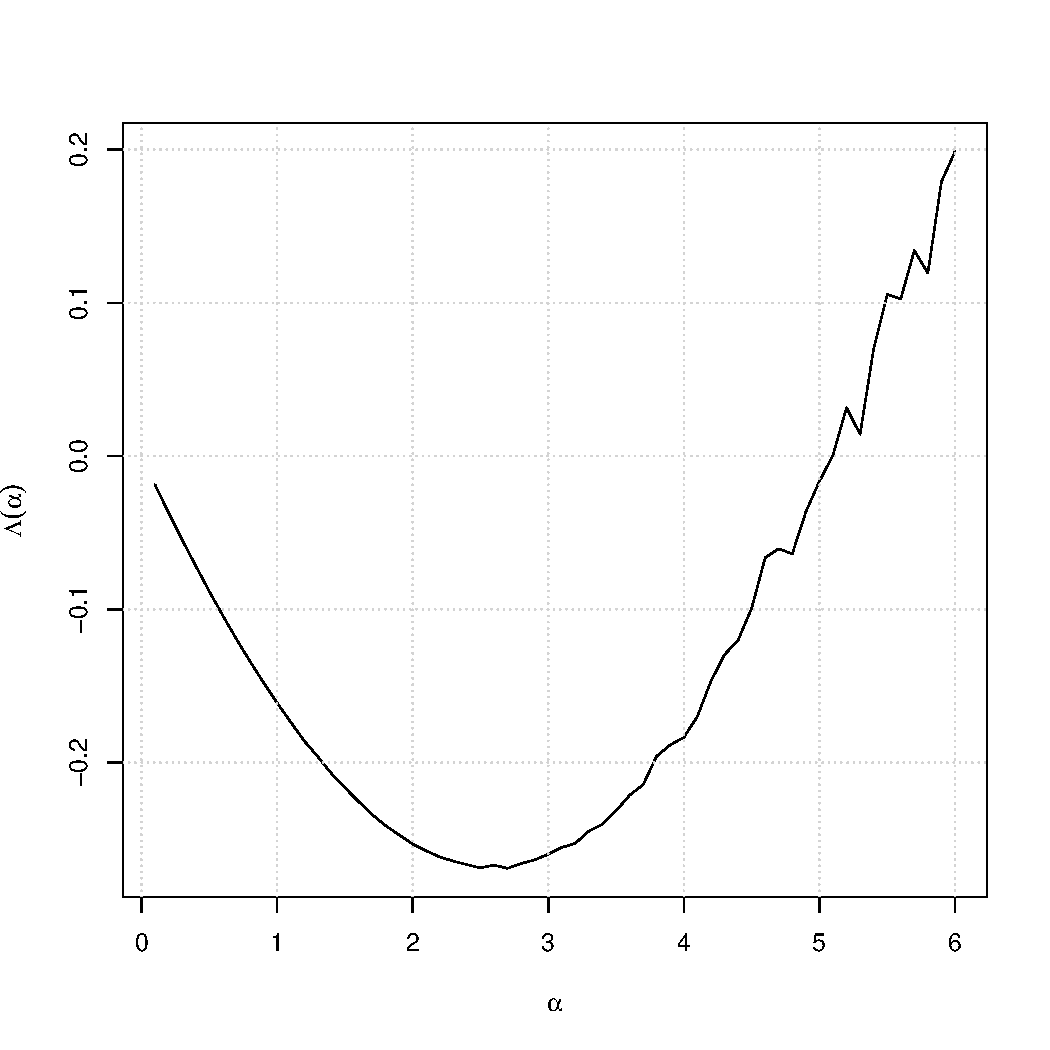
\includegraphics[width=\textwidth]{SP500_xi.pdf}
  \end{minipage}\hfill
  \begin{minipage}{0.5\linewidth}
    \centering
    $r_\xi(x)$ corresponding to $\xi$
    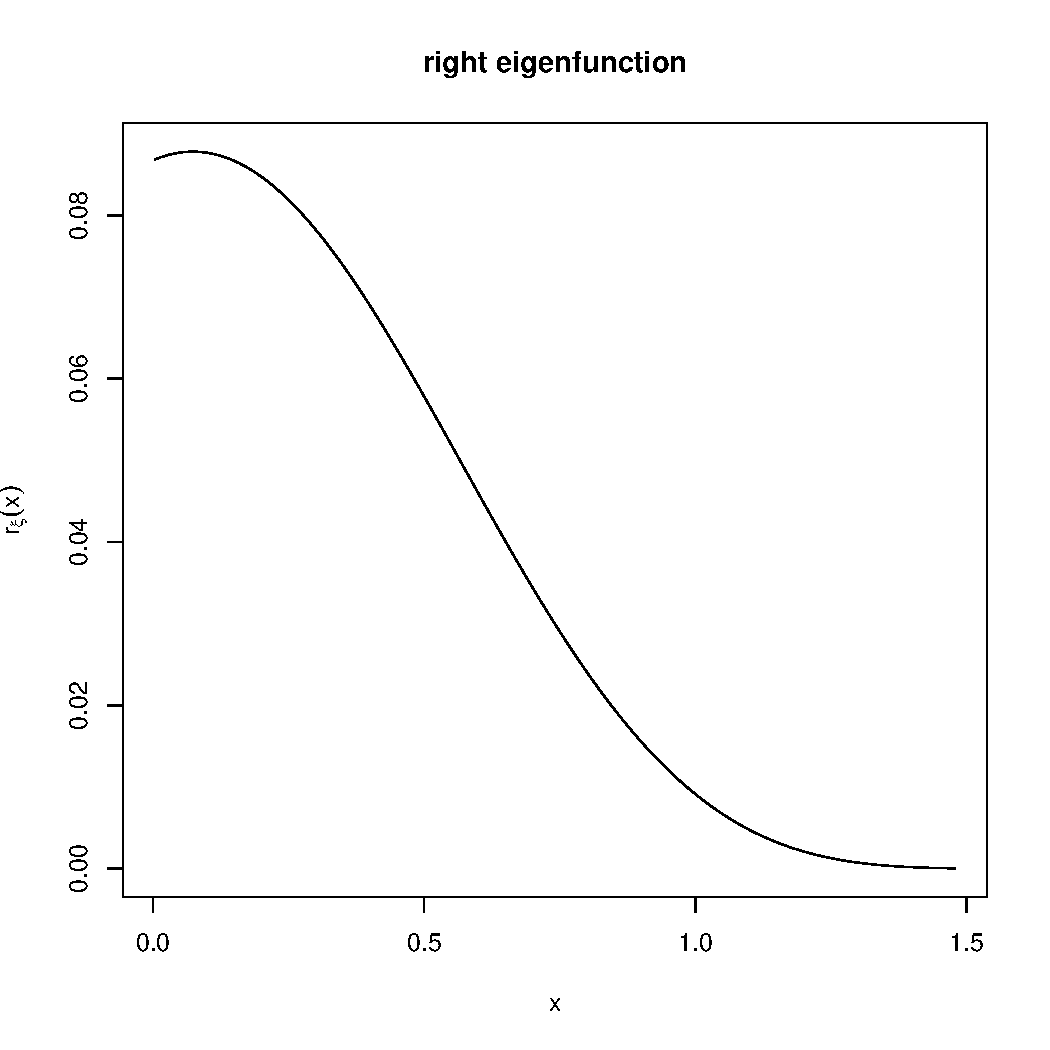
\includegraphics[width=\textwidth]{SP500_r.pdf}
  \end{minipage}
  
  
\end{itemize}

\subsubsection{DAX}
\begin{itemize}
\item GARCH(1, 1)
  When modeled as a GARCH(1, 1) process, the DAX return series
  has the coefficients as shown in the following equation
  \[
  \sigma_t^2 = 0.06 R_{t-1}^2 + 0.92 \sigma_{t-1}^2 + 3.1 \times 10^{-6}
  \]
  The tail index of the stationary distribution of $\sigma_t^2$ is
  estimated at 6.4269. The Hill estimator of this
  sequence is computed at 6.6020.
  % as the Hill plot in figure
  % \ref{fig:DAX_var_HillPlot} suggests.
  % \begin{figure}[htb!]
  %   \centering
  %   \includegraphics[scale=0.4]{DAX_var_HillPlot.pdf}    
  %   \caption{DAX $\sigma_t^2$ Hill Plot}
  %   \label{fig:DAX_var_HillPlot}
  % \end{figure}

\item GARCH(2, 1)
  When fitted to a GARCH(2, 1) process, the DAX return series has the following model
  \[
  \sigma_t^2 = 0.027 R_{t-1}^2 + 0.042 R_{t-2}^2 + 0.897 \sigma_{t-1}^2 + 4.0 \times 10^{-6}
  \]
  The algorithm with its current implementation has difficulty to
  estimate $\Lambda(\alpha)$ as $\alpha$ becomes large. This is shown
  in the figure below:
  \begin{figure}[htb!]
    \centering
    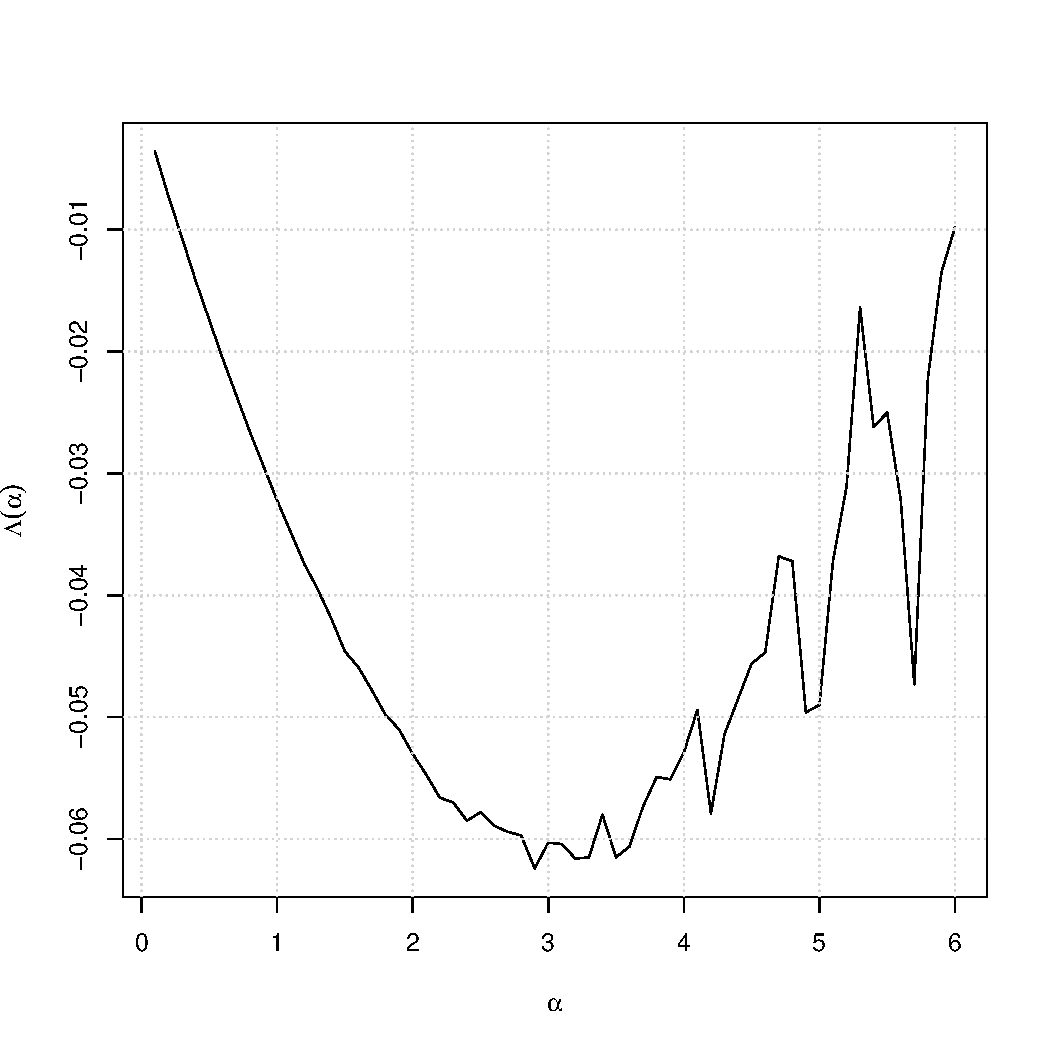
\includegraphics[width=\textwidth]{DAX_xi.pdf}
    \caption{$\Lambda(\alpha)$ estimates for DAX}
    \label{fig:DAX_garch21_tailindex}
  \end{figure}
  The estimated values of $\Lambda(\alpha)$ are listed table \ref{tab:DAX_garch21_tail_index}.
    \begin{table}[htb!]
    \centering
    \begin{tabular}{l|l|l|l||l|l|l|l}
      $\alpha$ & $\Lambda(\alpha)$ & err. & rel. err. & $\alpha$ & $\Lambda(\alpha)$ & err. & rel. err. \\
      \hline
      0.1000 & -0.0036 & 0.0009 & 0.2535 & 3.1000 & -0.0604 & 0.2027 & 3.3558 \\
      0.2000 & -0.0073 & 0.0017 & 0.2340 & 3.2000 & -0.0616 & 0.2585 & 4.1940 \\
      0.3000 & -0.0107 & 0.0020 & 0.1903 & 3.3000 & -0.0615 & 0.2669 & 4.3419 \\
      0.4000 & -0.0142 & 0.0025 & 0.1763 & 3.4000 & -0.0580 & 0.3232 & 5.5729 \\
      0.5000 & -0.0174 & 0.0027 & 0.1531 & 3.5000 & -0.0615 & 0.3719 & 6.0467 \\
      0.6000 & -0.0206 & 0.0030 & 0.1445 & 3.6000 & -0.0606 & 0.3794 & 6.2604 \\
      0.7000 & -0.0236 & 0.0038 & 0.1624 & 3.7000 & -0.0573 & 0.4485 & 7.8213 \\
      0.8000 & -0.0266 & 0.0050 & 0.1884 & 3.8000 & -0.0549 & 0.5345 & 9.7438 \\
      0.9000 & -0.0294 & 0.0073 & 0.2469 & 3.9000 & -0.0551 & 0.5655 & 10.2685 \\
      1.0000 & -0.0322 & 0.0089 & 0.2774 & 4.0000 & -0.0529 & 0.6865 & 12.9826 \\
      1.1000 & -0.0348 & 0.0109 & 0.3127 & 4.1000 & -0.0494 & 0.7077 & 14.3304 \\
      1.2000 & -0.0374 & 0.0146 & 0.3904 & 4.2000 & -0.0579 & 0.7418 & 12.8088 \\
      1.3000 & -0.0395 & 0.0178 & 0.4515 & 4.3000 & -0.0514 & 0.8021 & 15.6075 \\
      1.4000 & -0.0419 & 0.0218 & 0.5210 & 4.4000 & -0.0485 & 0.9369 & 19.3079 \\
      1.5000 & -0.0446 & 0.0260 & 0.5821 & 4.5000 & -0.0456 & 0.9525 & 20.8980 \\
      1.6000 & -0.0459 & 0.0304 & 0.6634 & 4.6000 & -0.0447 & 1.0402 & 23.2610 \\
      1.7000 & -0.0478 & 0.0356 & 0.7443 & 4.7000 & -0.0368 & 1.0678 & 28.9796 \\
      1.8000 & -0.0498 & 0.0421 & 0.8452 & 4.8000 & -0.0372 & 1.1068 & 29.7502 \\
      1.9000 & -0.0510 & 0.0482 & 0.9443 & 4.9000 & -0.0496 & 1.1848 & 23.8698 \\
      2.0000 & -0.0530 & 0.0543 & 1.0236 & 5.0000 & -0.0490 & 1.1304 & 23.0528 \\
      2.1000 & -0.0547 & 0.0650 & 1.1877 & 5.1000 & -0.0372 & 1.3674 & 36.7623 \\
      2.2000 & -0.0566 & 0.0713 & 1.2610 & 5.2000 & -0.0311 & 1.3533 & 43.5658 \\
      2.3000 & -0.0570 & 0.0820 & 1.4393 & 5.3000 & -0.0164 & 1.3191 & 80.2003 \\
      2.4000 & -0.0585 & 0.0914 & 1.5631 & 5.4000 & -0.0262 & 1.4752 & 56.2897 \\
      2.5000 & -0.0578 & 0.1070 & 1.8514 & 5.5000 & -0.0250 & 1.3379 & 53.5797 \\
      2.6000 & -0.0589 & 0.1163 & 1.9759 & 5.6000 & -0.0322 & 1.4219 & 44.1810 \\
      2.7000 & -0.0594 & 0.1302 & 2.1913 & 5.7000 & -0.0473 & 1.3915 & 29.4468 \\
      2.8000 & -0.0597 & 0.1516 & 2.5405 & 5.8000 & -0.0222 & 1.6773 & 75.3996 \\
      2.9000 & -0.0624 & 0.1663 & 2.6664 & 5.9000 & -0.0135 & 1.4893 & 110.0806 \\
      3.0000 & -0.0603 & 0.1877 & 3.1148 & 6.0000 & -0.0098 & 1.5522 & 158.6270
    \end{tabular}
    \caption{DAX: $\Lambda(\alpha)$ around $\alpha = \xi$. N = 400, K = 40000}
    \label{tab:DAX_garch21_tail_index}
  \end{table}


  %% \begin{minipage}{0.5\linewidth}
  %%   \centering
  %%   $\Lambda(\alpha)$
  %%   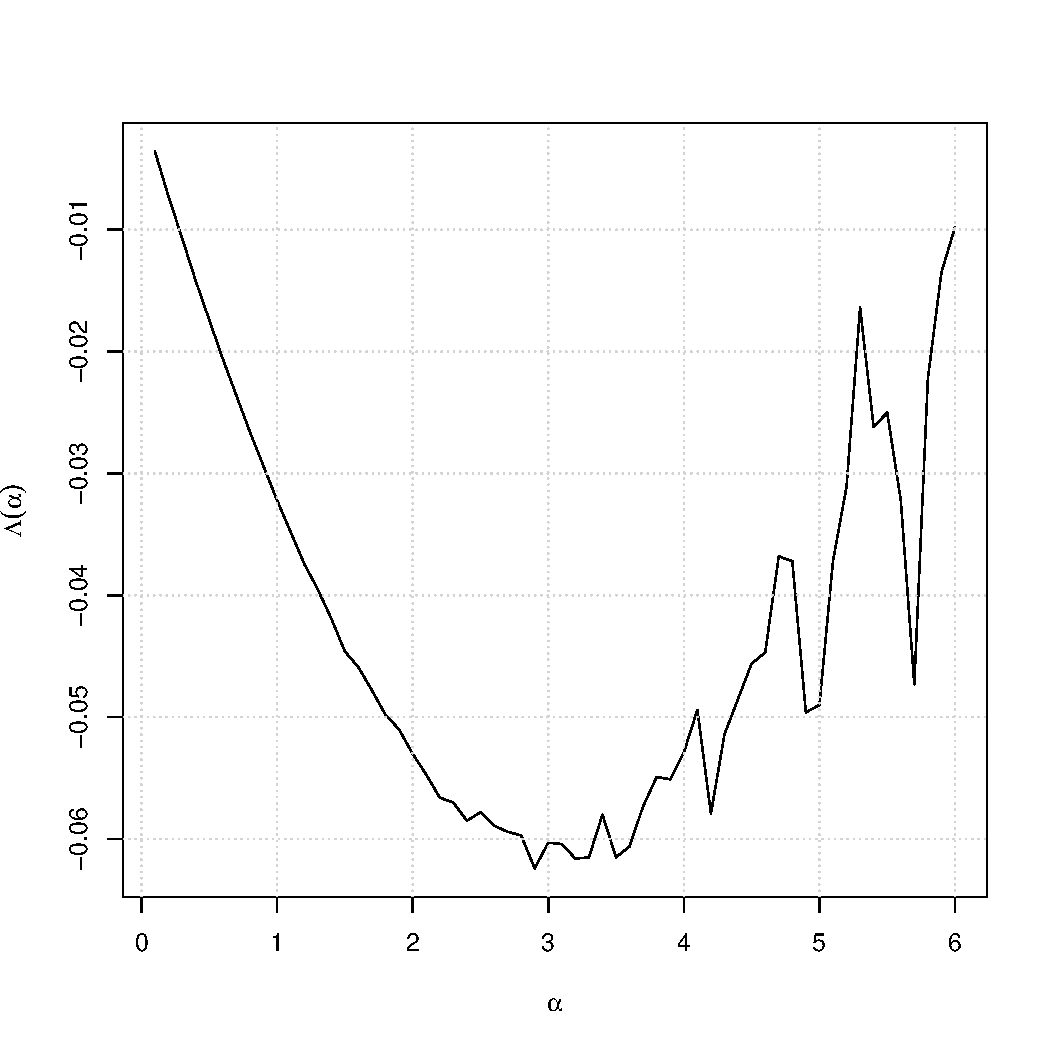
\includegraphics[width=\textwidth]{DAX_xi.pdf}
  %% \end{minipage}\hfill
  %% \begin{minipage}{0.5\linewidth}
  %%   \centering
  %%   $r_\xi(x)$ corresponding to $\xi$
  %%   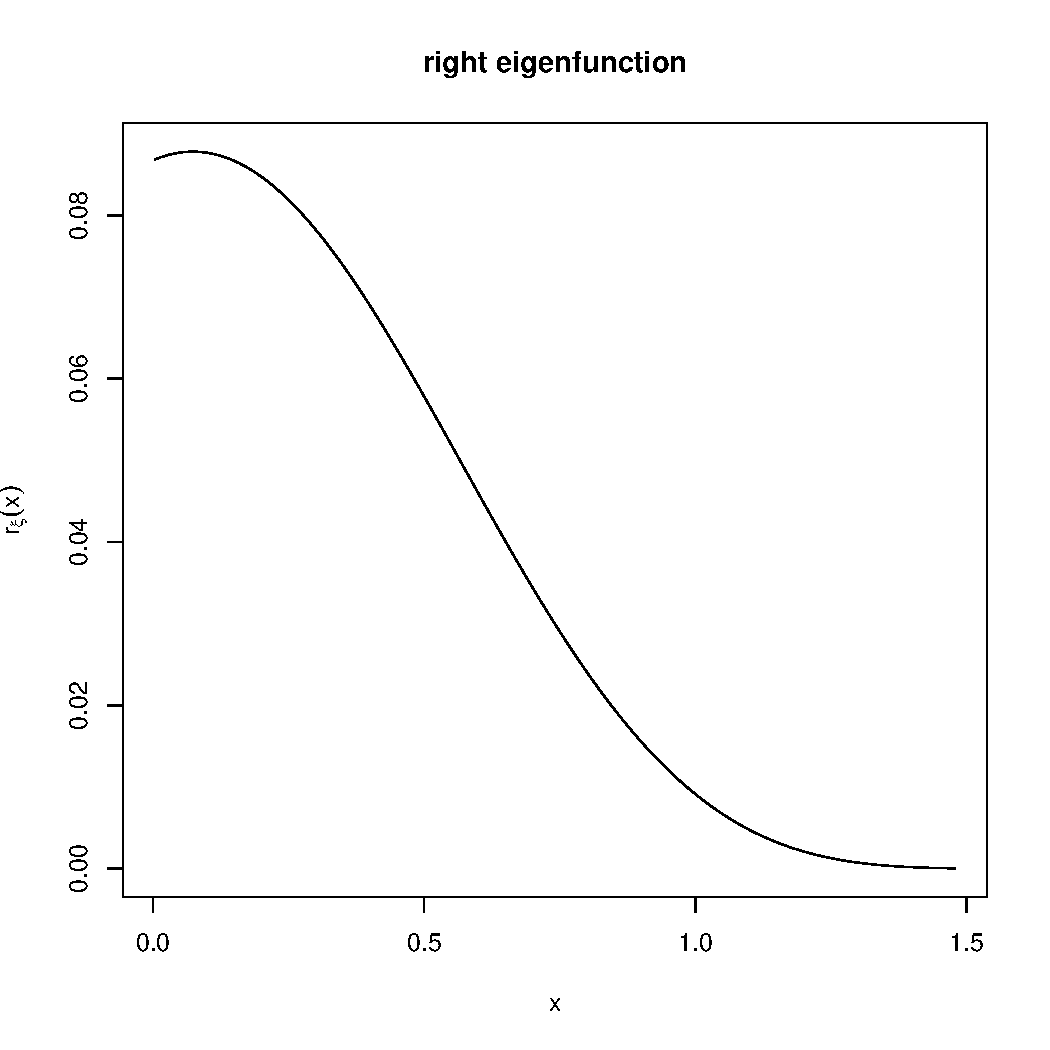
\includegraphics[width=\textwidth]{SP500_r.pdf}
  %% \end{minipage}

  % \begin{table}[htb!]
  %   \centering
  %   \begin{tabular}{c|c|c|c}
  %     $\alpha$ & $\Lambda(\alpha)$ & abs. err. & rel. err. \\
  %     \hline
  %     0.1000 & -0.0017 & 0.0026 & 1.5402 \\
  %     0.2000 &  0.0009 & 0.0053 & 6.1829 \\
  %     0.3000 &  0.0077 & 0.0075 & 0.9712 \\
  %     0.4000 &  0.0192 & 0.0096 & 0.4975 \\
  %     0.5000 &  0.0355 & 0.0121 & 0.3411 \\
  %   \end{tabular}
  %   \caption{$\Lambda(\alpha)$ of DAX as GARCH(2,1)}
  %   \label{tab:DAX_garch21_Lambda}
  % \end{table}
  % The tail index is estimated at 0.1801.
\end{itemize}

\section{Evaluation of the right eigenfunction}

\section*{Acknowledgements}

% \begin{supplement}
% \sname{Supplement A}\label{suppA}
% \stitle{Title of the Supplement A}
% \slink[url]{http://www.e-publications.org/ims/support/dowload/imsart-ims.zip}
% \sdescription{Dum esset rex in
% accubitu suo, nardus mea dedit odorem suavitatis. Quoniam confortavit
% seras portarum tuarum, benedixit filiis tuis in te. Qui posuit fines tuos}
% \end{supplement}


% \begin{thebibliography}{9}

% \bibitem{r1}
% \textsc{Billingsley, P.} (1999). \textit{Convergence of
% Probability Measures}, 2nd ed.
% Wiley, New York.
% \MR{1700749}


% \bibitem{r2}
% \textsc{Bourbaki, N.}  (1966). \textit{General Topology}  \textbf{1}.
% Addison--Wesley, Reading, MA.

% \bibitem{r3}
% \textsc{Ethier, S. N.} and \textsc{Kurtz, T. G.} (1985).
% \textit{Markov Processes: Characterization and Convergence}.
% Wiley, New York.
% \MR{838085}

% \bibitem{r4}
% \textsc{Prokhorov, Yu.} (1956).
% Convergence of random processes and limit theorems in probability
% theory. \textit{Theory  Probab.  Appl.}
% \textbf{1} 157--214.
% \MR{84896}

% \end{thebibliography}

\bibliographystyle{unsrt}
\bibliography{../../thesis/econophysics}
\end{document}
